% =============================================================================
%  IIIT RAICHUR -- B.Tech PROJECT THESIS
%  Department of Computer Science and Engineering
%  -----------------------------------------------------------------------------
%  Project: Naukri_Guru — AI-Powered Job Automation Platform
%  Author:  Manvendra Pratap Singh (CS22B1054)
%  Guide:   Dr. Neha Agarwal, Assistant Professor
%  =============================================================================

\documentclass[12pt, a4paper, oneside]{report}

% ---------------------- PACKAGES ---------------------------------------------
\usepackage[utf8]{inputenc}
\usepackage[T1]{fontenc}
\usepackage{lmodern}
\usepackage[margin=1in, top=1.2in, bottom=1.2in]{geometry}
\usepackage{graphicx}
\usepackage{setspace}
\usepackage{titlesec}
\usepackage{tocloft}
\usepackage{fancyhdr}
\usepackage{booktabs}
\usepackage{longtable}
\usepackage{array}
\usepackage{tabularx}
\usepackage{multirow}
\usepackage{caption}
\usepackage{subcaption}
\usepackage{amsmath, amssymb}
\usepackage{xcolor}
\usepackage[hidelinks, breaklinks=true]{hyperref}
\usepackage{url}
\usepackage{enumitem}
\usepackage{float}
\usepackage{listings}
\usepackage{courier}

% ---------------------- CODE LISTING STYLE ------------------------------------
\lstset{
  basicstyle=\small\ttfamily,
  breaklines=true,
  frame=single,
  numbers=left,
  numberstyle=\tiny,
  keywordstyle=\color{blue},
  commentstyle=\color{gray},
  stringstyle=\color{red},
  showstringspaces=false,
  tabsize=4
}

% ---------------------- USER INPUTS -------------------------------------------
\newcommand{\thesisTitle}{Naukri\_Guru: An AI-Powered Platform for Automated Job Application, Lifecycle Tracking, and Recruiter Outreach on LinkedIn}
\newcommand{\thesisTitleDisplay}{NAUKRI\_GURU: AN AI-POWERED PLATFORM \\ FOR AUTOMATED JOB APPLICATION, \\ LIFECYCLE TRACKING, AND RECRUITER OUTREACH \\ ON LINKEDIN}
\newcommand{\studentName}{Manvendra Pratap Singh}
\newcommand{\rollNumber}{CS22B1054}
\newcommand{\supervisorName}{Dr.~Neha Agarwal, Assistant Professor}
\newcommand{\departmentName}{Computer Science and Engineering}
\newcommand{\submissionMonthYear}{May 2026}
\newcommand{\submissionLocation}{Raichur -- 584135}
\newcommand{\degreeName}{Bachelor of Technology}
\newcommand{\logoPath}{images/iiitr_logo.png}

% ---------------------- FORMATTING -------------------------------------------
\onehalfspacing

\titleformat{\chapter}[display]
  {\normalfont\huge\bfseries}{\chaptertitlename\ \thechapter}{20pt}{\Huge}
\titlespacing*{\chapter}{0pt}{-30pt}{30pt}

\pagestyle{fancy}
\fancyhf{}
\fancyfoot[C]{\thepage}
\renewcommand{\headrulewidth}{0pt}
\renewcommand{\footrulewidth}{0pt}

\fancypagestyle{plain}{%
  \fancyhf{}%
  \fancyfoot[C]{\thepage}%
  \renewcommand{\headrulewidth}{0pt}%
  \renewcommand{\footrulewidth}{0pt}%
}

\renewcommand{\cftchapfont}{\bfseries}
\renewcommand{\cftchappagefont}{\bfseries}

\newcommand{\frontmatterheading}[1]{%
  \begin{center}\Large\bfseries #1\end{center}
  \vspace{0.5cm}
}

\setlength{\parskip}{0.5em}
\setlength{\parindent}{1.5em}

% =============================================================================
\begin{document}

% ---------------------- TITLE PAGE -------------------------------------------
\begin{titlepage}
    \centering
    \thispagestyle{empty}
    \vspace*{0.2cm}

    {\Large\bfseries \thesisTitleDisplay \par}
    \vspace{0.8cm}

    {\normalsize A Project Report Submitted \par}
    {\normalsize in Partial Fulfilment of the Requirements \par}
    {\normalsize for the Degree of \par}
    \vspace{0.5cm}

    {\large\bfseries \MakeUppercase{\degreeName} \par}
    \vspace{0.3cm}

    {\normalsize in \par}
    \vspace{0.2cm}

    {\large\bfseries \MakeUppercase{\departmentName} \par}
    \vspace{0.5cm}

    {\normalsize\itshape by \par}
    \vspace{0.3cm}

    {\normalsize\bfseries \studentName{} (Roll No.~\rollNumber) \par}
    \vspace{0.5cm}

    \includegraphics[width=1\textwidth]{\logoPath}\par
    \vspace{0.5cm}

    {\normalsize\itshape to \par}
    \vspace{0.2cm}

    {\normalsize\bfseries DEPARTMENT OF \MakeUppercase{\departmentName} \par}
    {\normalsize\bfseries INDIAN INSTITUTE OF INFORMATION TECHNOLOGY \par}
    {\normalsize\bfseries RAICHUR-584135, INDIA \par}
    \vspace{0.4cm}

    {\normalsize\itshape \submissionMonthYear \par}

\end{titlepage}

% ---------------------- FRONT MATTER -----------------------------------------
\pagenumbering{roman}
\setcounter{page}{2}

% ---------------------- DECLARATION ------------------------------------------
\clearpage
\thispagestyle{plain}
\frontmatterheading{DECLARATION}
\addcontentsline{toc}{chapter}{Declaration}

\noindent I \textbf{\MakeUppercase{\studentName}} (Roll Number: \rollNumber) hereby
declare that, this report entitled ``\textit{\thesisTitle}'' submitted to
Indian Institute of Information Technology Raichur towards partial requirement
of \degreeName{} in \departmentName{} is an original work carried out by me
under the supervision of Mentor, \supervisorName{} and has not formed the
basis for the award of any degree or diploma, in this or any other institution
or university. I have sincerely tried to uphold the academic ethics and
honesty. Whenever an external information or statement or result is used then,
that have been duly acknowledged and cited.

\vspace{2.5cm}
\noindent
\begin{minipage}[t]{0.5\textwidth}
\submissionLocation \\
\submissionMonthYear
\end{minipage}
\hfill
\begin{minipage}[t]{0.4\textwidth}
\raggedleft
\studentName \\
Roll No.~\rollNumber
\end{minipage}

% ---------------------- CERTIFICATE ------------------------------------------
\clearpage
\thispagestyle{plain}
\frontmatterheading{CERTIFICATE}
\addcontentsline{toc}{chapter}{Certificate}

\noindent This is to certify that the work contained in this project report
entitled ``\textit{\thesisTitle}'' submitted by \textbf{\studentName} (Roll
No: \rollNumber) to the Indian Institute of Information Technology Raichur
towards partial requirement of \degreeName{} in \departmentName{} has been
carried out by him under my supervision and that it has not been submitted
elsewhere for the award of any degree.

\vspace{3cm}
\noindent
\begin{minipage}[t]{0.5\textwidth}
\submissionLocation \\
\submissionMonthYear
\end{minipage}
\hfill
\begin{minipage}[t]{0.4\textwidth}
\raggedleft
(\supervisorName) \\
Project Supervisor
\end{minipage}

% ---------------------- ABSTRACT ---------------------------------------------
\clearpage
\thispagestyle{plain}
\frontmatterheading{ABSTRACT}
\addcontentsline{toc}{chapter}{Abstract}

Job hunting in the contemporary digital landscape demands considerable manual effort, as candidates routinely submit hundreds of applications through online portals while simultaneously tracking outcomes and engaging with recruiters. This report introduces \textbf{Naukri\_Guru}, an intelligent job automation platform engineered to streamline the entire LinkedIn application lifecycle through browser automation, artificial intelligence, and structured data management. The platform operates on a five-layer modular architecture comprising a user interface layer, an orchestration engine, an intelligence layer with support for multiple AI providers, a stealth browser automation layer, and a SQLite-backed persistence layer.

The system automates job discovery, role suitability evaluation through a heuristic confidence scoring engine, and application submission via LinkedIn's Easy Apply mechanism. A three-tier question answering cascade---combining statically configured personal data, a persistent memory store, and generative AI providers (Google Gemini, OpenAI, and DeepSeek) protected by a safety guard function---enables fully autonomous form completion. Beyond LinkedIn, the platform incorporates an Indeed job scraper that discovers and archives relevant positions for manual review. Post-application lifecycle management is achieved through Gmail IMAP synchronization, which classifies recruiter emails and matches them to stored applications, while a cold email outreach pipeline facilitates proactive recruiter engagement with AI-generated personalized messages.

Operational evaluation across twenty-three automation sessions demonstrates that the platform processes over eight hundred job listings, achieves an application success rate exceeding eighty-seven percent after server-side verification, and reduces per-application time by approximately ninety percent compared to manual effort. The memory-based question answering system converges toward near-autonomous operation within eight to nine sessions, progressively eliminating the need for human intervention in form completion.

% ---------------------- TABLE OF CONTENTS ------------------------------------
\clearpage
\tableofcontents
\listoffigures
\addcontentsline{toc}{chapter}{List of Figures}
\listoftables
\addcontentsline{toc}{chapter}{List of Tables}

\clearpage
\pagenumbering{arabic}
\setcounter{page}{1}

% =============================================================================
% CHAPTER 1: INTRODUCTION
% =============================================================================
\chapter{Introduction}
\label{chap:introduction}

Over the past decade the manner in which job seekers and employers connect has shifted decisively toward online platforms. Professional networking services, foremost among them LinkedIn, have emerged as the dominant channel through which millions of positions are advertised and filled each year. LinkedIn's own disclosures indicate a registered base exceeding nine hundred million members across more than two hundred countries, with tens of millions of companies maintaining active recruitment presences on the platform \cite{ref1}. For candidates entering competitive fields---particularly those in software engineering, data science, and allied technology disciplines---the sheer volume of available openings creates a paradox: while opportunities are abundant, the administrative burden of identifying suitable roles, completing application forms, and monitoring outcomes consumes a disproportionate share of the job seeker's time and cognitive energy.

This project addresses the inefficiency inherent in repetitive job application workflows by developing \textbf{Naukri\_Guru}, an AI-powered automation platform that converts LinkedIn's ``Easy Apply'' process into a largely autonomous pipeline. Complementing this core capability, the system also integrates an Indeed job scraper that discovers and archives relevant listings from a second major job portal, thereby broadening the candidate's visibility across the employment landscape. Unlike simplistic macro recorders or rigid browser scripts, Naukri\_Guru employs a layered software design that incorporates intelligent decision-making, persistent learning, structured data storage, email-based lifecycle tracking, and recruiter outreach---collectively transforming a tedious manual process into an efficient, data-driven operation.

The subsequent sections of this chapter describe the specific problems that motivated the development of Naukri\_Guru, articulate the significance of the proposed solution, define the boundaries of the implementation, and highlight the distinctive contributions of this work relative to existing tools.

\section{Problem Statement}
\label{sec:problem-statement}

Candidates pursuing technology roles encounter a set of interrelated obstacles that collectively render the application process slow, repetitive, and prone to errors:

\begin{itemize}
    \item \textbf{Application Volume Demands:} An engineering graduate actively searching for employment may need to submit between two hundred and five hundred applications before securing an acceptable offer. Even through LinkedIn's streamlined Easy Apply mechanism, each submission requires reading the job description, interacting with multi-step modal forms, uploading a resume, and answering screening questions---a sequence that consumes three to five minutes per application when performed manually.
    \item \textbf{Redundant Question Answering:} The screening questions embedded within LinkedIn's Easy Apply modals overlap substantially across employers. Queries regarding years of professional experience, visa sponsorship eligibility, salary expectations, notice period, and location preferences recur in nearly every application, forcing candidates to provide identical or near-identical responses hundreds of times.
    \item \textbf{Absence of Intelligent Pre-Screening:} Although LinkedIn offers basic search filters, it does not prevent candidates from encountering and spending time on fundamentally mismatched listings---senior positions appearing in entry-level searches, roles demanding security clearances that the candidate cannot obtain, or openings at companies the candidate has already decided to avoid.
    \item \textbf{Fragmented Outcome Tracking:} Once an application has been submitted, there exists no centralized mechanism for monitoring which companies have responded, which applications have been silently passed over, and which have progressed to interview stages. Recruiter communications arrive through email, LinkedIn notifications, and third-party applicant tracking systems, requiring tedious manual consolidation.
\end{itemize}

\section{Project Significance}
\label{sec:project-significance}

The value of this project stems from its comprehensive approach to automating the job application lifecycle, extending well beyond what existing tools offer individually:

\begin{itemize}
    \item \textbf{Dramatic Time Reduction:} Automated application submission compresses the per-application effort from three to five minutes of manual interaction to roughly fifteen to twenty seconds of machine-driven execution. Across a session involving one hundred candidate listings and five to seven actual submissions, this translates to a cumulative saving exceeding thirty minutes.
    \item \textbf{Heuristic Suitability Assessment:} Before committing to an application, the platform's confidence scoring engine evaluates each job description against the candidate's profile. The algorithm considers keyword relevance, seniority indicators, degree requirements, and experience thresholds, assigning a quantitative suitability score on a zero-to-one-hundred scale.
    \item \textbf{Adaptive Learning Through Memory:} The question answering module maintains a persistent JSON-based memory store that records previously provided answers. Over successive sessions, the fraction of questions requiring either AI assistance or human input diminishes steadily, and the system approaches fully autonomous form completion within approximately five sessions.
    \item \textbf{Multi-Portal Job Discovery:} In addition to LinkedIn, the Indeed scraper module broadens the candidate's search surface by collecting and archiving relevant job listings from Indeed, presenting them in a structured spreadsheet format with colour-coded source attribution for manual review and follow-up.
    \item \textbf{Unified Lifecycle Visibility:} Gmail IMAP synchronization enables the platform to automatically detect and classify recruiter responses---including interview invitations, online assessment links, rejections, and offers---and update the application database accordingly, providing a consolidated view of the candidate's entire job search trajectory.
\end{itemize}

\section{Scope of Work}
\label{sec:scope}

The implementation encompasses the following major components:

\begin{itemize}
    \item \textbf{Stealth Browser Automation Engine:} A Chrome-based automation layer utilizing \texttt{undetected-chromedriver} and Selenium WebDriver, operating within an isolated browser profile to circumvent LinkedIn's anti-bot defences. A Selenium Manager fallback guarantees driver resolution even when the primary stealth library encounters compatibility issues.
    \item \textbf{Job Discovery and Intelligent Filtering Pipeline:} A configurable search and filter mechanism that discovers LinkedIn job listings based on keywords, location, experience level, and additional parameters, then subjects each listing to a multi-factor filtering funnel encompassing blacklist checking, confidence scoring, seniority detection, and bad-word filtering.
    \item \textbf{AI-Assisted Question Answering Module:} A cascading answer resolution system that sequentially consults static configuration mappings, a persistent JSON memory cache, and one of three supported AI providers (Google Gemini, OpenAI, DeepSeek), with a dedicated safety guard function that intercepts and overrides AI-generated responses for personally sensitive question categories.
    \item \textbf{Indeed Job Scraper:} A collect-only scraping module that navigates Indeed's search interface, extracts job card metadata (title, company, location, URL), applies relevance filtering through configurable bad-word lists, and persists results to a unified job store with source attribution.
    \item \textbf{Application Lifecycle and Data Persistence Layer:} A SQLite-backed storage architecture with tables for applications, recruiters, lifecycle events, cold emails, and failure logs, complemented by CSV and XLSX export capabilities with colour-coded formatting and Gmail IMAP synchronization for automated status updates.
    \item \textbf{Cold Email Outreach Pipeline:} An automated recruiter engagement system that discovers recruiter contact details, generates personalised cold emails using AI, validates email trustworthiness through a multi-signal scoring mechanism, and dispatches messages via authenticated SMTP with rate limiting and duplicate prevention.
\end{itemize}

The platform targets the Windows operating system and is implemented in Python 3.10+. The modular architecture facilitates future extension to additional job portals beyond the currently supported LinkedIn and Indeed integrations.

\section{Objectives}
\label{sec:objectives}

The principal objectives of this project are:

\begin{enumerate}
    \item To architect and implement a stealth browser automation engine capable of navigating LinkedIn's dynamically rendered job search interface and Easy Apply modals without triggering anti-bot detection.
    \item To develop a confidence scoring algorithm that quantitatively assesses the suitability of each discovered job listing relative to the candidate's profile, producing a score on a zero-to-one-hundred scale.
    \item To construct a multi-tier question answering system that combines static configuration, persistent memory, and generative AI to autonomously fill LinkedIn screening questions with contextually correct responses.
    \item To build an Indeed job scraper that discovers, filters, and archives relevant job listings from Indeed for manual review, with source-attributed persistence in a unified job store.
    \item To implement a structured SQLite persistence layer that records every application attempt, failure event, and lifecycle transition with complete audit trails and deduplication guarantees.
    \item To integrate Gmail IMAP synchronization that classifies recruiter emails by application status and matches them to stored applications using multi-signal evidence scoring.
    \item To engineer a cold email outreach pipeline with AI-generated personalised content, recruiter email trust validation, and SMTP delivery with sender reputation safeguards.
\end{enumerate}

\section{Novelty}
\label{sec:novelty}

Although several open-source and commercial LinkedIn automation tools exist, Naukri\_Guru contributes a number of distinctive elements that set it apart from prior work:

\begin{itemize}
    \item \textbf{Multi-Provider AI with Safety Guard Architecture:} Rather than depending on a single language model, the platform supports three AI providers through a unified interface. A dedicated guard function (\texttt{guard\_ai\_answer}) intercepts every AI response and overrides it with verified personal data whenever the question matches a safety-critical pattern---such as queries about graduation year, salary, or contact number---thereby preventing the AI from fabricating sensitive personal details.
    \item \textbf{Persistent Memory with Skill-Specific Experience Routing:} The memory module differentiates between general questions and skill-specific experience queries (for instance, ``How many years of React experience do you have?'') through a keyword detection mechanism, routing each to specialised handlers that maintain per-skill answer caches independent of the general memory store.
    \item \textbf{Post-Submission Verification Protocol:} Instead of assuming success after clicking the submit button, the system inspects the resulting DOM for LinkedIn's confirmation markers (such as ``application submitted'' text or the presence of a ``Done'' button) and refuses to persist the application record unless positive verification is obtained, thereby eliminating phantom entries from the tracking database.
    \item \textbf{Dual-Portal Job Discovery:} The integration of an Indeed scraper alongside the LinkedIn automation engine provides cross-platform job visibility within a single tool, with a unified job store (\texttt{job\_store.py}) that deduplicates across sources and produces colour-coded XLSX reports for streamlined manual review.
    \item \textbf{Runtime Batch Traceability:} Every automation session generates a unique \texttt{runtime\_batch\_id} that tags all database records, lifecycle events, and cold email dispatches produced during that session, enabling per-session audit trails and retrospective analysis.
\end{itemize}

The convergence of these capabilities produces an automation platform that functions not as a mechanical click-replay bot, but as an intelligent agent capable of adapting to diverse application forms, learning from user interactions, operating across multiple job portals, and maintaining rigorous data integrity throughout its operational lifecycle.


% =============================================================================
% CHAPTER 2: LITERATURE SURVEY
% =============================================================================
\chapter{Literature Survey}
\label{chap:literature}

This chapter surveys the existing body of work across three domains that underpin the Naukri\_Guru platform: job application automation tools, browser automation and anti-detection technologies, and AI-assisted form filling systems. For each domain, representative approaches are examined, their strengths and weaknesses are identified, and the manner in which Naukri\_Guru extends or departs from them is articulated. The objective is to situate the project within the broader landscape of employment technology and intelligent web automation.

\section{Existing Approaches -- Job Application Automation Tools}
\label{sec:category-a}

The expansion of web-based recruitment has given rise to a range of tools designed to alleviate the manual labour associated with job applications. These solutions span commercial subscription services, open-source automation scripts, and resume optimization utilities.

\subsection{LazyApply}
LazyApply is a subscription-based automation service supporting several job platforms, including LinkedIn, Indeed, and ZipRecruiter \cite{ref2}. It provides a browser extension that pre-populates profile data and submits applications on the user's behalf. Despite its multi-platform reach, LazyApply stores all user data on remote servers, relies on template-based question answering without generative AI fallback, and provides no local persistence or post-application lifecycle tracking. Its subscription pricing model also creates an ongoing cost barrier for individual users.

\subsection{EasyApplyBot (Open-Source)}
EasyApplyBot is a community-maintained Python project built on Selenium that automates LinkedIn's Easy Apply workflow \cite{ref3}. The tool supports basic search configuration and fills form fields using hardcoded values. However, it lacks several capabilities that limit its practical utility: there is no persistent memory for previously answered questions, no heuristic scoring to filter unsuitable listings, no post-application tracking or lifecycle management, and no stealth measures beyond standard Selenium, leaving it susceptible to LinkedIn's bot-detection heuristics.

\subsection{JobScan}
JobScan is a commercial resume analysis tool that compares a candidate's resume against individual job descriptions and generates a compatibility score \cite{ref4}. It excels at keyword analysis and Applicant Tracking System (ATS) compatibility assessment. However, it operates strictly as a pre-application advisory service and does not automate any part of the submission, tracking, or outreach workflow.

\subsection{Differentiation of Our Approach}
Naukri\_Guru distinguishes itself from these tools across several dimensions:

\begin{itemize}
    \item In contrast to LazyApply, all data in Naukri\_Guru remains on the user's local machine within a SQLite database, ensuring privacy and eliminating subscription costs.
    \item Unlike EasyApplyBot, this system implements a three-tier answer resolution cascade (configuration, memory, and AI with guard), heuristic confidence scoring, post-submission verification, and dual-portal job discovery through the Indeed scraper.
    \item While JobScan provides pre-application advice, Naukri\_Guru automates the entire lifecycle from discovery through submission to recruiter engagement.
\end{itemize}

\begin{table}[H]
\centering
\caption{Comparison of Job Application Automation Tools}
\label{tab:cat-a-comparison}
\small
\begin{tabularx}{\textwidth}{|l|l|l|X|X|}
\hline
\textbf{Tool} & \textbf{Type} & \textbf{Year} & \textbf{Key Features} & \textbf{Limitations} \\
\hline
LazyApply \cite{ref2} & Commercial SaaS & 2021 & Multi-platform, browser extension, cloud profile & No local storage, subscription cost, no AI Q\&A \\
\hline
EasyApplyBot \cite{ref3} & Open-source & 2022 & Python/Selenium, Easy Apply automation & No memory, no scoring, no anti-detection, no lifecycle \\
\hline
JobScan \cite{ref4} & Commercial SaaS & 2018 & Resume-JD matching, ATS optimization & Advisory only, no submission automation \\
\hline
\textbf{Naukri\_Guru} & Open-source & 2026 & AI Q\&A with guard, confidence scoring, Gmail sync, cold email, Indeed scraper, SQLite persistence & LinkedIn-primary, Windows-optimised \\
\hline
\end{tabularx}
\end{table}

\section{Existing Approaches -- Browser Automation and Anti-Detection}
\label{sec:category-b}

Browser automation frameworks constitute the technical foundation upon which web-based application tools are constructed. The principal challenge extends beyond driving browser interactions to doing so without being identified as automated traffic by the target platform.

\subsection{Selenium WebDriver}
Selenium WebDriver remains the most widely adopted framework for programmatic browser control, offering a language-agnostic API compatible with Chrome, Firefox, Edge, and Safari through platform-specific driver binaries \cite{ref5}. Its maturity and extensive documentation make it a natural starting point for automation projects. However, unmodified Selenium usage exposes detectable fingerprints---most notably the \texttt{navigator.webdriver} JavaScript property being set to \texttt{true}---which sophisticated platforms exploit to identify and block automated sessions.

\subsection{Puppeteer and Playwright}
Puppeteer, maintained by Google, and Playwright, maintained by Microsoft, are Node.js-based automation frameworks that communicate with browsers via the Chrome DevTools Protocol \cite{ref6}. They provide superior performance for JavaScript-intensive single-page applications and offer built-in stealth capabilities. Their primary drawback for Python-centric projects is the Node.js runtime requirement, which introduces a language ecosystem barrier. Moreover, their stealth features are designed for general-purpose evasion rather than being tuned for the specific detection mechanisms employed by LinkedIn.

\subsection{Undetected ChromeDriver}
The \texttt{undetected-chromedriver} library is a Python package that patches the standard ChromeDriver binary to eliminate known automation indicators \cite{ref7}. It modifies browser fingerprints, suppresses the \texttt{webdriver} flag, and randomises certain browser properties to simulate organic user traffic. This library is specifically designed for scenarios where standard Selenium triggers anti-bot protections, making it well-suited for LinkedIn automation.

\subsection{Differentiation of Our Approach}
Naukri\_Guru's browser architecture combines multiple anti-detection strategies in a fault-tolerant configuration:

\begin{itemize}
    \item \textbf{Primary Path:} The system employs \texttt{undetected-chromedriver} with automatic detection of the installed Chrome version, ensuring driver-browser version alignment and eliminating the common ChromeDriver mismatch failure.
    \item \textbf{Fallback Path:} If stealth startup fails, the platform automatically falls back to Selenium Manager for driver resolution, maintaining operational continuity regardless of the stealth library's compatibility state.
    \item \textbf{Profile Isolation:} All automation executes within a dedicated directory (\texttt{C:\textbackslash Naukri\_Guru\_Profile}), physically separated from the user's personal Chrome profiles to prevent cookie contamination and session conflicts.
\end{itemize}

\begin{table}[H]
\centering
\caption{Comparison of Browser Automation Frameworks}
\label{tab:cat-b-comparison}
\small
\begin{tabularx}{\textwidth}{|l|X|X|}
\hline
\textbf{Framework} & \textbf{Key Features} & \textbf{Limitations} \\
\hline
Selenium \cite{ref5} & Cross-browser, multi-language, mature ecosystem & Detectable fingerprints, no built-in stealth \\
\hline
Puppeteer \cite{ref6} & DevTools Protocol, stealth plugins, fast rendering & Node.js only, not Python-native \\
\hline
undetected-chromedriver \cite{ref7} & Python-native, patches automation flags, version matching & Chrome-only, occasional lag behind Chrome updates \\
\hline
\end{tabularx}
\end{table}

\section{Existing Approaches -- AI-Assisted Form Filling and NLP}
\label{sec:category-c}

Applying natural language processing and large language models to automated form completion represents an emerging research direction at the intersection of task-oriented dialogue systems and web automation.

\subsection{GPT-Based Auto-Fill Systems}
Recent explorations have leveraged OpenAI's GPT models for automated form completion, wherein the language model generates contextually relevant responses based on question text and user profile data \cite{ref8}. These approaches demonstrate competence with open-ended textual questions but encounter difficulties with structured inputs---dropdowns, radio buttons, and checkboxes---where the response must precisely match one of a finite set of options. A further concern is that purely AI-driven approaches risk fabricating personal information when the model lacks adequate context about the user.

\subsection{Resume Parsing and Information Extraction}
Platforms such as Affinda and Sovren deploy NLP techniques to extract structured data from unstructured resume documents \cite{ref9}. These parsers identify entities including educational history, work experience, skills, and contact details. While useful for populating candidate profiles, they do not address the challenge of real-time question answering during dynamic form navigation, where questions are encountered sequentially and require immediate, contextually appropriate responses.

\subsection{Differentiation of Our Approach}
Naukri\_Guru's intelligence layer overcomes the shortcomings of purely AI-driven approaches through a cascading answer resolution strategy:

\begin{itemize}
    \item \textbf{Configuration First:} Frequently asked personal questions (name, phone number, address, experience) are mapped to statically configured values, guaranteeing correctness without involving any AI component.
    \item \textbf{Memory Second:} Previously answered questions are cached in a persistent JSON file (\texttt{memory.json}) with normalised question keys, supporting both exact and fuzzy recall for recurring questions across sessions.
    \item \textbf{AI Third with Safety Guards:} When neither configuration nor memory yields an answer, the system queries the selected AI provider. The generated response passes through \texttt{guard\_ai\_answer()}, which inspects the question for safety-critical patterns (graduation year, experience, salary, phone number, location) and replaces the AI's output with the user's configured value whenever a match is detected.
\end{itemize}

\begin{table}[H]
\centering
\caption{Comparison of AI-Assisted Form Filling Approaches}
\label{tab:cat-c-comparison}
\small
\begin{tabularx}{\textwidth}{|l|X|X|X|}
\hline
\textbf{Approach} & \textbf{Key Features} & \textbf{Methodology} & \textbf{Limitations} \\
\hline
GPT Auto-Fill \cite{ref8} & Context-aware generation & Prompt-based LLM Q\&A & Hallucinated data, no structured inputs \\
\hline
Resume Parsers \cite{ref9} & Structured extraction & NER, pattern matching & Static only, no real-time Q\&A \\
\hline
\textbf{Naukri\_Guru} & Config $\to$ Memory $\to$ AI with guard & Multi-tier with safety overrides & AI dependency for novel questions \\
\hline
\end{tabularx}
\end{table}

The literature review reveals that while the constituent technologies---browser automation, AI-powered form filling, and application tracking---have been explored independently, no existing solution weaves all of these capabilities together with the depth, robustness, and cross-portal coverage that Naukri\_Guru provides. The nearest prior work, EasyApplyBot, addresses only the browser automation aspect without intelligence, memory, lifecycle tracking, or multi-portal discovery. This project fills that gap by delivering a unified, intelligent, and self-improving automation platform.


% =============================================================================
% CHAPTER 3: METHODOLOGY
% =============================================================================
\chapter{Methodology}
\label{chap:methodology}

This chapter elaborates the technical methodology underpinning Naukri\_Guru, presenting the system architecture, execution pipeline, and the internal design of each functional module. The discussion is structured around the five-phase execution pipeline that the platform follows during each operational session, with detailed attention to the algorithms, data structures, and integration patterns employed at each stage.

\section{Problem Restatement}
\label{sec:problem-restatement}

The central technical challenge can be decomposed into four interconnected sub-problems:

\begin{itemize}
    \item \textbf{Reliable Browser Interaction:} Navigating LinkedIn's dynamic, JavaScript-heavy interface---including modal dialogue boxes, paginated listing grids, and asynchronously loaded form elements---without triggering anti-bot detection or encountering stale DOM references.
    \item \textbf{Contextual Decision Making:} Determining, for each discovered listing, whether it aligns with the candidate's profile based on the job description content, and generating appropriate responses to screening questions that differ in format and semantics across employers.
    \item \textbf{Cross-Portal Discovery:} Extending the search surface beyond LinkedIn by scraping job listings from Indeed, filtering them for relevance, and persisting them in a unified data store alongside LinkedIn application records.
    \item \textbf{Data Integrity and Lifecycle Management:} Maintaining a consistent, deduplicated record of all application attempts and their outcomes across multiple data sources (LinkedIn confirmation, Gmail emails, Indeed scraping) with atomic persistence guarantees.
\end{itemize}

\section{Overall Approach}
\label{sec:overall-approach}

Naukri\_Guru's execution follows a five-phase pipeline that mirrors the natural job application workflow while introducing automation and intelligence at every stage:

\begin{itemize}
    \item \textbf{Phase 1 -- Pre-Flight and Synchronization:} Validation of configuration files, initialisation and maintenance of the SQLite database, and Gmail IMAP lifecycle synchronization. This phase establishes a consistent system state before any browser interaction commences.
    \item \textbf{Phase 2 -- Stealth Browser Initialization:} Chrome launch with anti-detection countermeasures, profile isolation, stale lock file removal, and LinkedIn authentication. The browser is configured to operate within an isolated automation profile that does not interfere with the user's personal browsing sessions.
    \item \textbf{Phase 3 -- Job Discovery and Filtering:} Keyword-based job search on LinkedIn, application of built-in filters, extraction of job card metadata, blacklist checking, confidence scoring, seniority filtering, bad-word filtering, and session-level company-title deduplication. This phase functions as a multi-stage funnel that progressively narrows the candidate pool to suitable positions.
    \item \textbf{Phase 4 -- Automated Application and Indeed Scraping:} For LinkedIn, this phase involves Easy Apply modal navigation, multi-format question answering (text, select, radio, textarea, checkbox), resume upload, follow-company toggle, submission with verification, and failure handling. For Indeed, this phase discovers job listings through configured search terms, applies bad-word filtering, and persists qualifying records to the unified job store.
    \item \textbf{Phase 5 -- Post-Application Processing:} SQLite persistence, CSV and XLSX export with colour coding, cold email outreach to recruiters, and session summary reporting. This phase ensures all application data is durably stored and recruiter visibility is enhanced through proactive outreach.
\end{itemize}

\section{System Block Diagram}
\label{sec:block-diagram}

The block diagram (Figure~\ref{fig:block-diagram}) depicts the high-level layered architecture, illustrating five functional layers and the data flow among them. The User Interface Layer produces human-readable outputs through a Flask dashboard and Excel reports. The Orchestration Layer houses the main engine (\texttt{runAiBot.py}), the scheduled runner, and the Indeed scraper. The Intelligence Layer encapsulates the AI connectors, confidence scoring engine, and persistent memory. The Automation Layer manages the stealth Chrome browser and Gmail IMAP connection. The Persistence Layer stores all data in SQLite, with file-based job description storage and CSV/XLSX compatibility exports.

\begin{figure}[H]
    \centering
    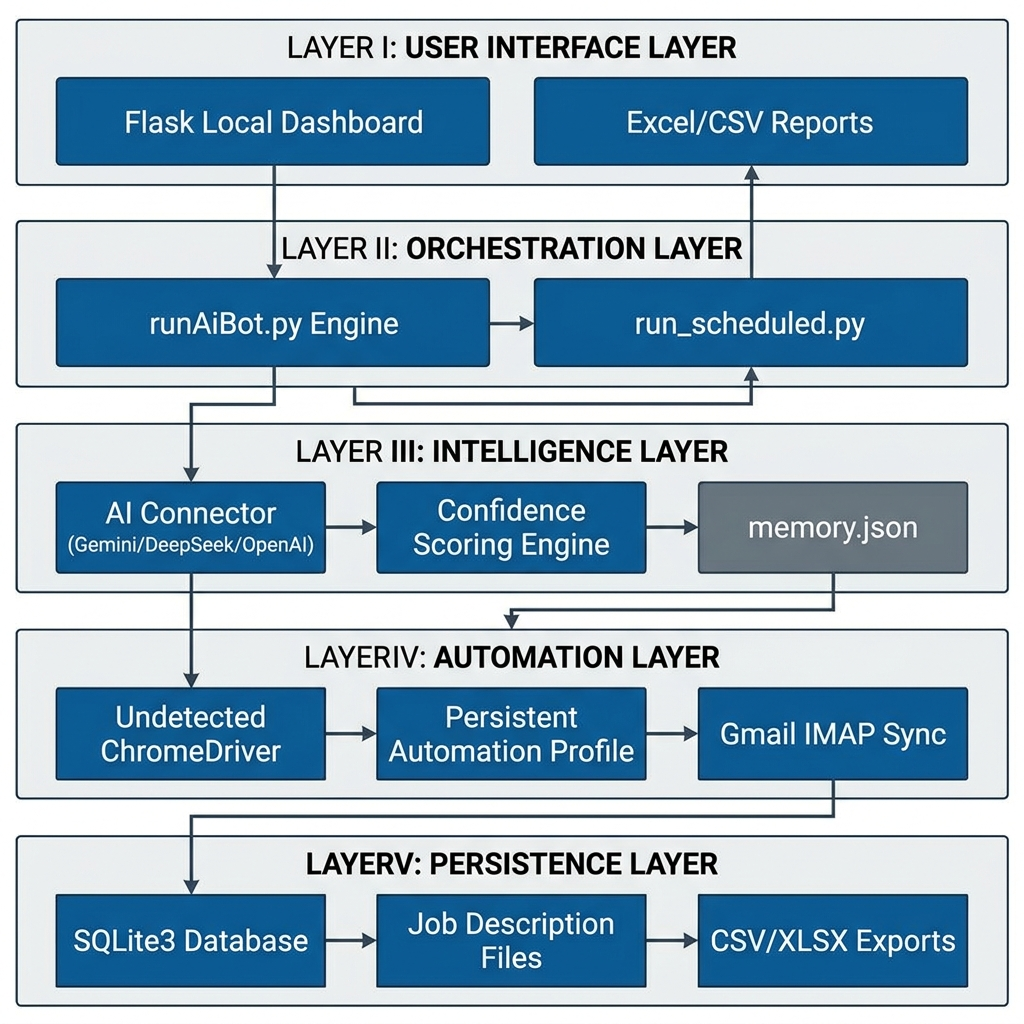
\includegraphics[width=0.9\textwidth]{images/block_diagram.png}
    \caption{System Block Diagram -- Five-Layer Architecture of Naukri\_Guru}
    \label{fig:block-diagram}
\end{figure}

Each layer communicates with its adjacent layers through well-defined Python function interfaces, enabling independent testing and modification of individual components without disrupting the remainder of the system.

\section{Architecture}
\label{sec:architecture}

The overall software architecture is shown in Figure~\ref{fig:architecture}. The system is organised as a modular Python application with the following component responsibilities:

\begin{figure}[H]
    \centering
    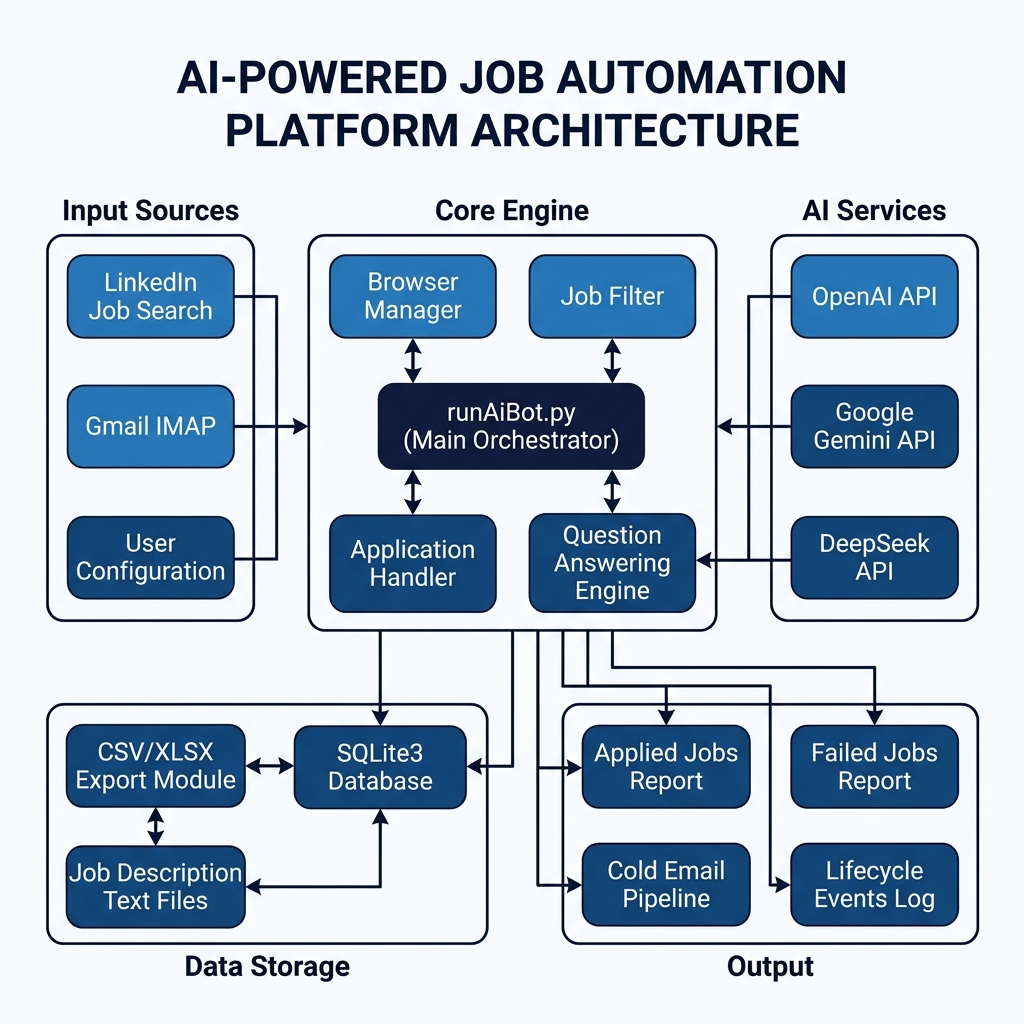
\includegraphics[width=0.9\textwidth]{images/architecture.png}
    \caption{Software Architecture -- Component Interaction Diagram}
    \label{fig:architecture}
\end{figure}

The architecture adheres to a decoupled design in which the orchestration engine (\texttt{runAiBot.py}) coordinates between independent modules:

\begin{itemize}
    \item \texttt{modules/browser/} --- Chrome session management and driver initialisation with version detection.
    \item \texttt{modules/ai/} --- AI provider connectors for OpenAI, Gemini, and DeepSeek with prompt engineering.
    \item \texttt{modules/email/} --- Gmail IMAP authentication, email fetching, status classification, and application matching.
    \item \texttt{modules/cold\_email/} --- Recruiter email discovery, personalised email generation, SMTP delivery, and tracking.
    \item \texttt{modules/indeed/} --- Indeed job card extraction, bad-word filtering, and unified job store persistence.
    \item \texttt{modules/storage.py} --- SQLite database operations, schema management, and CSV/XLSX export.
    \item \texttt{modules/memory.py} --- Persistent question-answer cache with normalised key matching and skill routing.
    \item \texttt{modules/job\_store.py} --- Unified multi-source job store with deduplication and XLSX colour coding.
    \item \texttt{modules/validator.py} --- Environment and pipeline validation utilities.
    \item \texttt{modules/runtime\_context.py} --- Runtime batch identifier generation for session traceability.
    \item \texttt{config/} --- User configuration files for personal details, search parameters, API secrets, and behavioural settings.
\end{itemize}

\section{Module One: Stealth Browser Automation Engine}
\label{sec:module-one}

The browser automation engine is responsible for launching an isolated Chrome instance capable of navigating LinkedIn without triggering anti-bot protections. The initialisation sequence, illustrated in Figure~\ref{fig:module1}, follows a fault-tolerant startup protocol.

\begin{figure}[H]
    \centering
    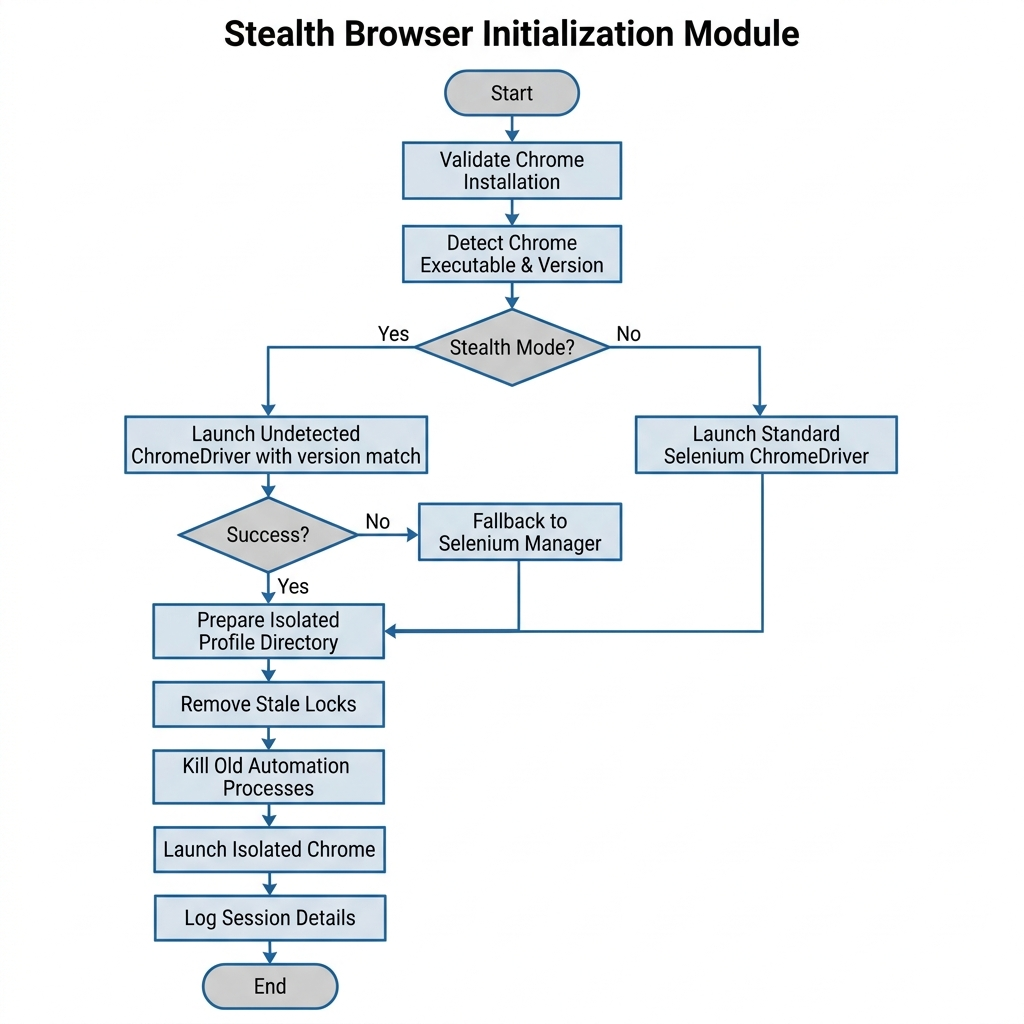
\includegraphics[width=0.9\textwidth]{images/module1_flow.png}
    \caption{Module One -- Stealth Browser Initialization Process Flow}
    \label{fig:module1}
\end{figure}

The key technical decisions within this module are as follows:

\textbf{Chrome Version Detection:} The system identifies the installed Chrome executable and extracts its major version number. This value is supplied to \texttt{undetected-chromedriver} to guarantee that the ChromeDriver binary matches the installed browser, avoiding the prevalent ``ChromeDriver version mismatch'' error that arises when Chrome auto-updates in the background.

\textbf{Profile Isolation:} Every automation session utilises a dedicated profile directory (\texttt{C:\textbackslash Naukri\_Guru\_Profile}) that is physically separated from the user's personal Chrome profiles. Prior to each launch, the system purges stale lock files (\texttt{SingletonLock}, \texttt{SingletonCookie}) from the profile directory and terminates any Chrome processes previously attached to this path. This prevents ``user data directory is already in use'' errors across successive runs.

\textbf{Fallback Strategy:} Should the \texttt{undetected-chromedriver} launch fail---as can occur when the library lags behind a Chrome update---the system automatically falls back to standard Selenium with WebDriver Manager for driver resolution. This dual-path approach ensures operational continuity regardless of the stealth library's compatibility state.

\textbf{Session Health Monitoring:} After launch, the system validates the browser session by checking \texttt{driver.current\_window\_handle}, scanning the page source for CAPTCHA checkpoint markers, and verifying LinkedIn's authentication state by inspecting for login-wall indicators.

\section{Module Two: Job Discovery and Intelligent Filtering}
\label{sec:module-two}

The job discovery module implements a multi-stage filtering funnel that progressively narrows the pool of job listings to only those that merit an application. The filtering process is depicted in Figure~\ref{fig:module2}.

\begin{figure}[H]
    \centering
    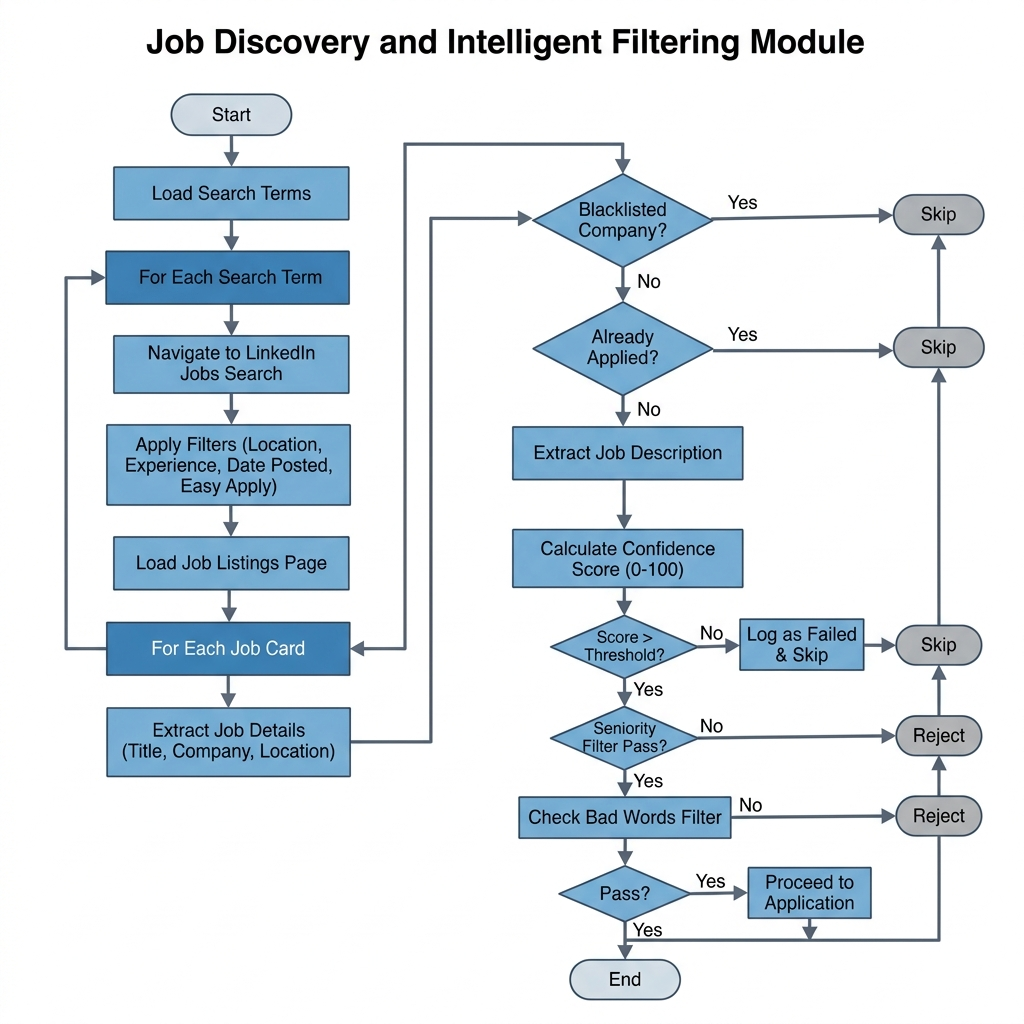
\includegraphics[width=0.9\textwidth]{images/module2_flow.png}
    \caption{Module Two -- Job Discovery and Intelligent Filtering Process Flow}
    \label{fig:module2}
\end{figure}

\textbf{Search and Filter Configuration:} The system iterates through a list of user-defined search terms (for example, ``Software Engineer'', ``Python Developer'', ``Machine Learning'') and navigates to LinkedIn's job search page for each term. It then applies a comprehensive set of filters: location, experience level, job type, work style (remote, hybrid, or on-site), date posted, and the Easy Apply filter. These parameters are drawn from \texttt{config/search.py} and applied through LinkedIn's ``All Filters'' modal.

\textbf{Job Card Extraction:} For each listing on the results page, the system extracts the job identifier (from the \texttt{data-occludable-job-id} attribute), position title, company name, work location, and work style. The extraction employs a cascading CSS selector strategy that tries multiple selectors for each field to accommodate LinkedIn's frequent DOM structure changes across A/B testing variants.

\textbf{Blacklist and Duplicate Checking:} Before proceeding with any application, the system verifies that the company does not appear in the user's blacklist (\texttt{about\_company\_bad\_words}), that the job identifier has not already been recorded in the SQLite database via \texttt{application\_exists()}, that the LinkedIn job card does not display an ``Applied'' badge, and that the company-title combination has not already been processed within the current session (session-level deduplication).

\textbf{Confidence Scoring:} The \texttt{calculate\_confidence\_score()} function evaluates the full job description text and produces a suitability score on a zero-to-one-hundred scale. The algorithm starts from a base score of sixty and applies additive adjustments for positive indicators (intern, fresher, Python) and subtractive adjustments for negative indicators (consulting, clearance, senior):

\begin{lstlisting}[language=Python, caption={Confidence Scoring Algorithm (Simplified)}, label={lst:confidence}]
def calculate_confidence_score(text):
    score = 60  # Base score
    text_lower = text.lower()
    # Positive indicators
    if 'intern' in text_lower: score += 20
    if 'fresher' in text_lower: score += 15
    if 'python' in text_lower: score += 10
    # Negative indicators
    if 'consulting' in text_lower: score -= 15
    if 'clearance' in text_lower: score -= 20
    return min(100, max(0, score))
\end{lstlisting}

\textbf{Seniority and Degree Filtering:} The \texttt{extract\_degree\_and\_seniority()} function uses regular expression pattern matching to detect advanced degree requirements (PhD, Doctorate) and high-seniority role indicators (Principal, Staff, Director, Architect) in both the job title and description. Listings matching these patterns are automatically bypassed with a logged justification.

\section{Module Three: Intelligent Question Answering}
\label{sec:module-three}

The question answering module constitutes the core intelligence component, responsible for autonomously filling LinkedIn's Easy Apply screening forms. The resolution process is illustrated in Figure~\ref{fig:module3}.

\begin{figure}[H]
    \centering
    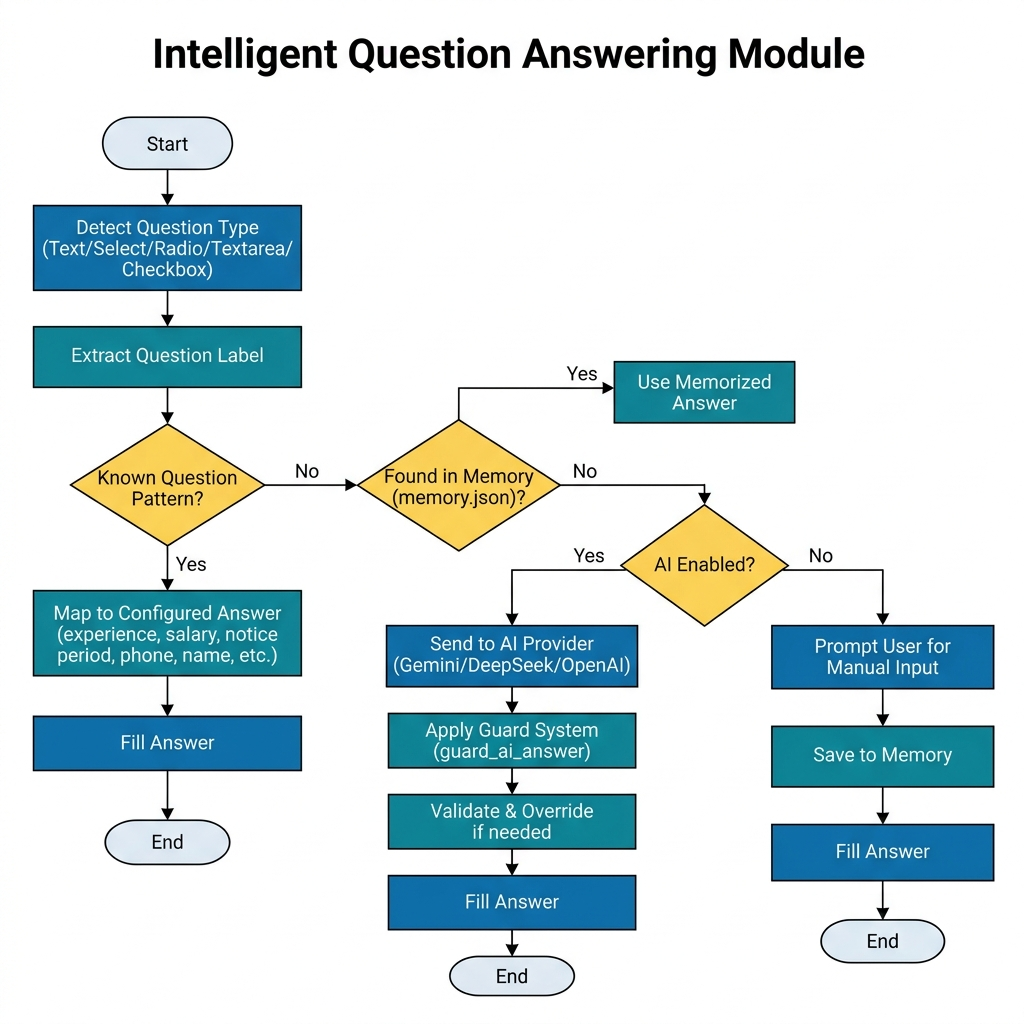
\includegraphics[width=0.9\textwidth]{images/module3_flow.png}
    \caption{Module Three -- Intelligent Question Answering Process Flow}
    \label{fig:module3}
\end{figure}

The module handles five distinct question formats:

\begin{enumerate}
    \item \textbf{Select Dropdowns:} Identified via \texttt{<select>} elements. The system extracts option texts and matches them against configured answers using bidirectional substring matching. For experience-related dropdowns, a dedicated \texttt{resolve\_experience\_select\_answer()} function ensures safe selection.
    \item \textbf{Radio Buttons:} Identified via \texttt{<fieldset>} elements with radio button components. Options are extracted with their labels and values. Matching follows configured preferences for citizenship, veteran status, disability status, and sponsorship questions.
    \item \textbf{Text Inputs:} Identified via \texttt{<input type="text">} elements. These accommodate the broadest variety of questions: experience years, phone number, name fields, address components, salary expectations, notice period, LinkedIn profile URL, and website links.
    \item \textbf{Textareas:} Identified via \texttt{<textarea>} elements. Typically used for summary or cover letter questions, these are populated using configured text or AI-generated content.
    \item \textbf{Checkboxes:} Identified via \texttt{<input type="checkbox">} elements. These are typically agreement or acknowledgement checkboxes and are automatically selected.
\end{enumerate}

\textbf{The Three-Tier Cascade:} For each encountered question, the answering priority follows this sequence:

\begin{enumerate}
    \item \textbf{Tier 1 -- Static Configuration:} Direct mapping from question label keywords to configured personal values. For instance, if the label contains ``phone'' or ``mobile'', the configured phone number is returned immediately.
    \item \textbf{Tier 2 -- Persistent Memory:} The system queries \texttt{memory.json} using normalised question keys (lowercased, stripped of punctuation, collapsed whitespace). Both exact and fuzzy matching (substring containment) are attempted.
    \item \textbf{Tier 3 -- AI with Guard:} If the preceding tiers fail, the question is dispatched to the configured AI provider. The AI's response passes through \texttt{guard\_ai\_answer()}, which checks whether the question matches any of eight safety-critical patterns (graduation year, experience, current CTC, desired salary, notice period, phone number, city/location, age) and overrides the AI response with the corresponding configured value upon detection.
\end{enumerate}

\textbf{Skill-Specific Experience Routing:} The \texttt{is\_skill\_specific\_experience\_question()} function identifies questions that ask about experience with a particular technology (for example, ``How many years of Python experience do you have?'') by checking for both experience keywords and a curated list of over thirty technology names. These questions are routed to a separate memory cache keyed by skill name, ensuring that the answer for ``Python experience'' remains independent of the answer for ``React experience.''

\section{Module Four: Application Lifecycle and Data Persistence}
\label{sec:module-four}

The data persistence module ensures that every application attempt, outcome, and subsequent lifecycle event is durably stored with complete audit trails. The persistence flow is shown in Figure~\ref{fig:module4}.

\begin{figure}[H]
    \centering
    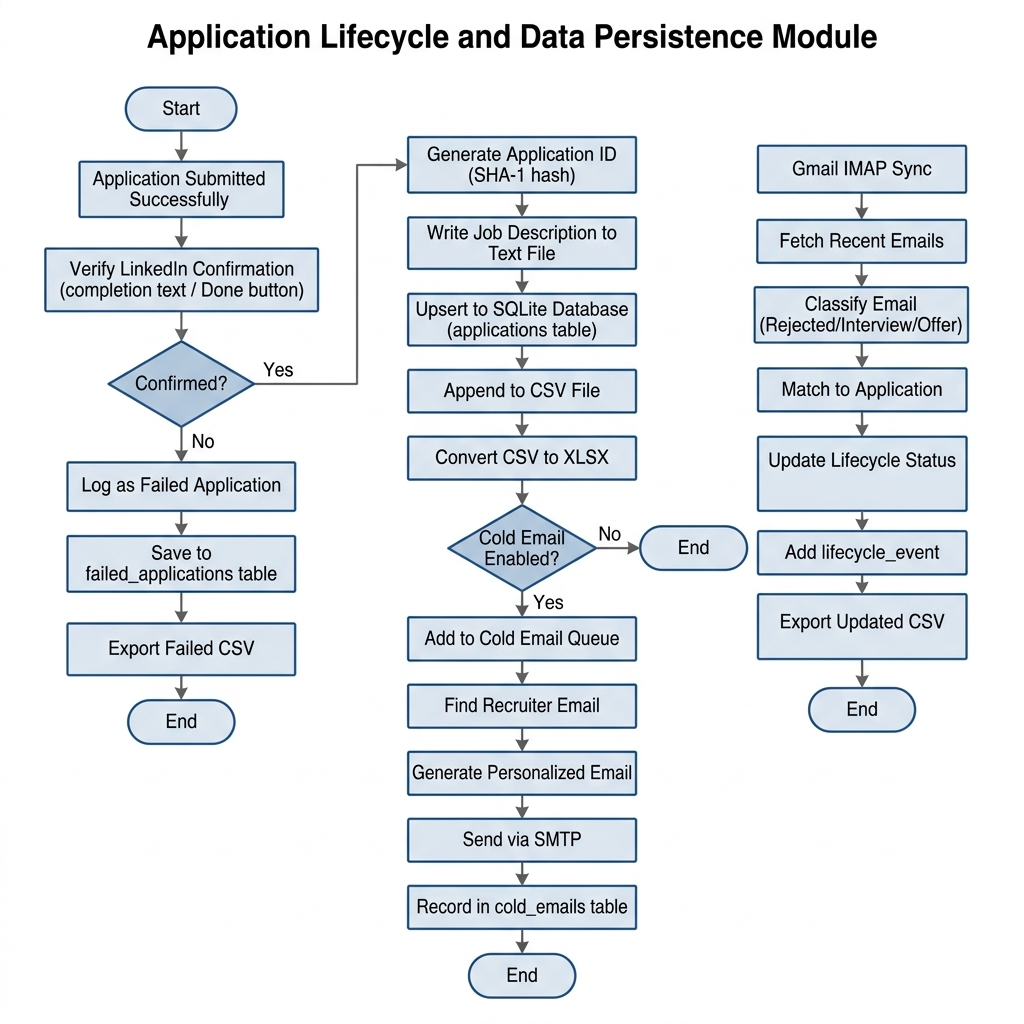
\includegraphics[width=0.9\textwidth]{images/module4_flow.png}
    \caption{Module Four -- Application Lifecycle and Data Persistence Flow}
    \label{fig:module4}
\end{figure}

\textbf{SQLite Schema Design:} The database (\texttt{data/naukri\_guru.sqlite3}) comprises the following tables:

\begin{itemize}
    \item \texttt{applications} --- Core application data with columns for job details, status tracking, cold email state, recruiter information, and runtime metadata.
    \item \texttt{failed\_applications} --- Records of application attempts that failed at any stage, preserving the failure reason and stack trace for diagnostic purposes.
    \item \texttt{lifecycle\_events} --- Timeline of status changes for each application, with source attribution (LinkedIn, Gmail, manual) and confidence scores.
    \item \texttt{recruiters} --- CRM-style storage of recruiter contact details extracted from LinkedIn job cards.
    \item \texttt{cold\_emails} --- Delivery tracking for outreach emails including SMTP status, timestamps, and error details.
\end{itemize}

\textbf{Application ID Generation:} Each application receives a deterministic identifier constructed by computing the SHA-1 hash of the concatenation of job identifier, job URL, title, company, and application date. The prefix \texttt{app\_} followed by the first sixteen hexadecimal characters of the hash produces a unique, reproducible identifier that enables deduplication across sessions.

\textbf{Post-Submission Verification:} After the submit button is clicked, the \texttt{verify\_easy\_apply\_submission()} function searches for LinkedIn's confirmation markers in both the modal and page content. It checks for phrases such as ``application submitted'', ``your application was sent'', and the presence of a ``Done'' button without a ``Submit application'' button. Only upon positive verification does the system persist the application record with a timestamp; otherwise, the attempt is logged as a failure with a diagnostic reason.

\textbf{Gmail IMAP Synchronization:} Before each automation session, the system connects to the user's Gmail account via IMAP and retrieves recent emails (configurable lookback period, default twenty days). Each email passes through a classification pipeline:

\begin{enumerate}
    \item \textbf{Sender Filtering:} Emails from low-trust domains (Glassdoor, Indeed, Naukri, job alert services) are discarded.
    \item \textbf{Status Classification:} A keyword-based classifier assigns each email a status (Interview Scheduled, OA Received, Rejected, Offer, and others) with a confidence score.
    \item \textbf{Application Matching:} The classified email is matched to a stored application using a multi-signal algorithm that considers exact job URL and identifier match, recruiter email and domain match, normalised company and title similarity, fuzzy text matching, and timing evidence.
    \item \textbf{Status Update:} If the match confidence exceeds the configured threshold (default 0.75) and the detected status has higher priority than the current status (per a defined priority ordering), the application record is updated and a lifecycle event is created.
\end{enumerate}

\textbf{Cold Email Pipeline:} The cold email outreach system operates on a queue model: after all applications in a session are completed, the system queries the database for applications with recruiter email addresses that have not yet received cold emails. For each eligible application, the recruiter email is validated through a trust scoring system, a personalised email is generated using the AI provider, the message is dispatched via authenticated SMTP with configurable inter-email delays, and the delivery outcome is recorded in both the applications and cold emails tables.

\section{Module Five: Indeed Job Scraper}
\label{sec:module-five}

The Indeed scraper operates in a collect-only mode: it discovers, filters, and archives job listings from Indeed without attempting automated applications. This design reflects the fact that Indeed's application flows typically redirect to external employer portals, making end-to-end automation impractical compared to LinkedIn's self-contained Easy Apply mechanism.

\textbf{Search and Navigation:} The scraper navigates to Indeed's search page for each configured search term and location combination. It waits for the results page to load, then extracts job card elements using CSS selectors defined in \texttt{modules/indeed/selectors.py}.

\textbf{Card Extraction:} For each job card, the scraper extracts the position title, company name, location, and job URL. The extraction uses a multi-selector strategy to accommodate Indeed's DOM variability.

\textbf{Relevance Filtering:} Each extracted listing is passed through a relevance filter that checks the job title and company name against the \texttt{bad\_words} and \texttt{about\_company\_bad\_words} lists from \texttt{config/search.py}. Listings containing blacklisted terms are discarded with a logged justification.

\textbf{Unified Job Store Persistence:} Qualifying records are saved to the unified job store via \texttt{modules/job\_store.py}. The job store implements deduplication based on a composite key of job identifier and source, preventing duplicate entries across sessions. The store generates both CSV and XLSX exports, with the XLSX version featuring colour-coded source attribution (distinct colours for LinkedIn and Indeed entries) and clickable hyperlinks for job URLs.

\textbf{Per-Term and Global Caps:} The scraper respects two configurable limits: \texttt{INDEED\_MAX\_JOBS\_PER\_TERM} (default ten) prevents any single search term from consuming the entire budget, while \texttt{INDEED\_MAX\_JOBS\_TO\_SCRAPE} (default ten) sets the global cap for the entire session.


% =============================================================================
% CHAPTER 4: CHALLENGES AND SOLUTIONS
% =============================================================================
\chapter{Challenges and Solutions}
\label{chap:challenges}

Building an automation platform that operates against a live, adversarial web service entails confronting a range of technical obstacles that span browser compatibility, DOM instability, AI reliability, and data integrity. This chapter documents the most significant challenges encountered during the development and operation of Naukri\_Guru and the engineering solutions devised to address them. Each challenge was observed during actual system operation and is reflected in the current codebase.

A consolidated summary of the major issues and their resolutions is presented in Table~\ref{tab:challenges}.

\begin{table}[H]
\centering
\caption{Major Implementation Challenges and Their Solutions}
\label{tab:challenges}
\begin{tabularx}{\textwidth}{|X|X|}
\hline
\textbf{Challenge} & \textbf{Solution} \\
\hline
ChromeDriver version mismatch after Chrome auto-updates causes startup failure
& Automatic Chrome version detection with matched \texttt{undetected-chromedriver} initialisation; Selenium Manager fallback when stealth startup fails \\
\hline
LinkedIn's Easy Apply modal DOM structure changes across A/B tests, causing element-not-found errors during form navigation
& Multi-selector cascading strategy: each UI element is targeted by three to five CSS selectors tried in priority order; modal detection uses five selectors with retry logic \\
\hline
``Review job post'' interstitial button mistakenly treated as ``Review application'' button, causing application abandonment
& Explicit handling of ``Continue applying'' interstitial screen before entering the question loop; prioritised exact match for ``Review your application'' over bare ``Review'' substring \\
\hline
Duplicate job listings appearing with different LinkedIn job IDs for the same position at the same company
& Session-level company-title deduplication set that prevents the same company-title combination from being processed twice within a single session \\
\hline
AI providers generating fabricated personal information (hallucinated phone numbers, incorrect salary figures)
& \texttt{guard\_ai\_answer()} safety layer that pattern-matches question labels and overrides AI responses with configured personal values for eight critical categories \\
\hline
Unknown questions causing application abandonment when no answer is available
& Persistent memory system with user prompt fallback; skill-specific experience routing; \texttt{UserCancelledException} for graceful skip without terminating the session \\
\hline
Daily Easy Apply limit reached mid-session causing subsequent applications to fail silently
& Detection of LinkedIn's ``exceeded the daily application limit'' inline feedback message; immediate session termination with summary report \\
\hline
Phantom ``Applied'' entries in the database when the submit action fires but LinkedIn does not actually process the submission
& \texttt{verify\_easy\_apply\_submission()} function inspecting modal and page content for five distinct confirmation markers before recording success \\
\hline
Indeed job results containing irrelevant positions due to loose keyword matching
& Integration of \texttt{bad\_words} and \texttt{about\_company\_bad\_words} filters from the LinkedIn configuration into the Indeed scraper pipeline \\
\hline
Cold email dispatched to invalid or untrustworthy recruiter email addresses, risking sender reputation damage
& Multi-signal trust scoring system; low-trust sender domain blacklist; recruiter email quarantine; rate-limited SMTP with configurable delays \\
\hline
\end{tabularx}
\end{table}

\textbf{ChromeDriver Version Mismatch:} This was the most frequently encountered operational issue during early development. Google Chrome updates silently in the background, and when the browser's major version (for example, 149) diverges from the ChromeDriver binary version (for example, 148), Selenium cannot establish a connection. The solution extracts the Chrome major version at runtime through subprocess calls to the Chrome executable, then passes this version to \texttt{undetected-chromedriver}'s constructor. If this approach fails, the system falls back to Selenium's integrated manager, which downloads the appropriate driver automatically.

\textbf{``Continue Applying'' Interstitial:} When LinkedIn detects a potential mismatch between the candidate's profile and a job listing, it presents an interstitial screen with ``Review job post'' and ``Continue applying'' buttons before displaying the actual application form. The system's button-matching logic initially interpreted ``Review job post'' as the final-step ``Review'' button, causing it to navigate away from the application flow. The fix introduces explicit detection of the ``Continue applying'' button immediately after modal acquisition, clicking it to proceed to the actual form, and modifies the ``Review'' search to prioritise the full ``Review your application'' text over bare substring matching.

\textbf{Session-Level Deduplication:} LinkedIn occasionally lists the same position at the same company with different job identifiers---typically representing different location variants of an identical role. The database-level deduplication, which checks by job identifier, fails to catch these near-duplicates. A session-level in-memory set tracking company-title pairs prevents the same position from being processed twice within a single run, without blocking genuinely different roles at the same company.

\textbf{Memory Learning Loop:} When the system encounters a question that cannot be answered through configuration or memory, it prompts the user with a GUI dialogue (using \texttt{pyautogui}) requesting the correct response. The answer is immediately stored in \texttt{memory.json} with a normalised key, category classification, confidence score, source attribution, and timestamp. Subsequent encounters of the same or similar question are handled automatically from memory, creating a progressive learning loop that converges toward fully autonomous operation within three to five sessions.


% =============================================================================
% CHAPTER 5: RESULTS AND DISCUSSION
% =============================================================================
\chapter{Results and Discussion}
\label{chap:results}

This chapter presents operational results obtained from running Naukri\_Guru across multiple automation sessions. The evaluation addresses three primary dimensions: the core LinkedIn application automation pipeline, the Gmail lifecycle synchronization accuracy, and the cold email outreach effectiveness. Additionally, results from the Indeed job scraping module are reported. All metrics are derived from actual system operation against real LinkedIn and Indeed job listings, with company names and recruiter identities anonymised where necessary.

\section{Application Automation Results}
\label{sec:result-set-1}

The LinkedIn automation engine was evaluated over a series of sessions targeting software engineering, data science, and machine learning roles.

\subsection{Session Execution Summary}
A representative session console output is displayed in Figure~\ref{fig:result1}. During a typical session, the system processes twenty-five to forty job listings per search term, applies the multi-stage filtering funnel, and submits five to seven Easy Apply applications. The per-application execution time---measured from the initial job card click to confirmed submission---averages fifteen to twenty seconds, compared to three to five minutes of manual effort.

\begin{figure}[H]
    \centering
    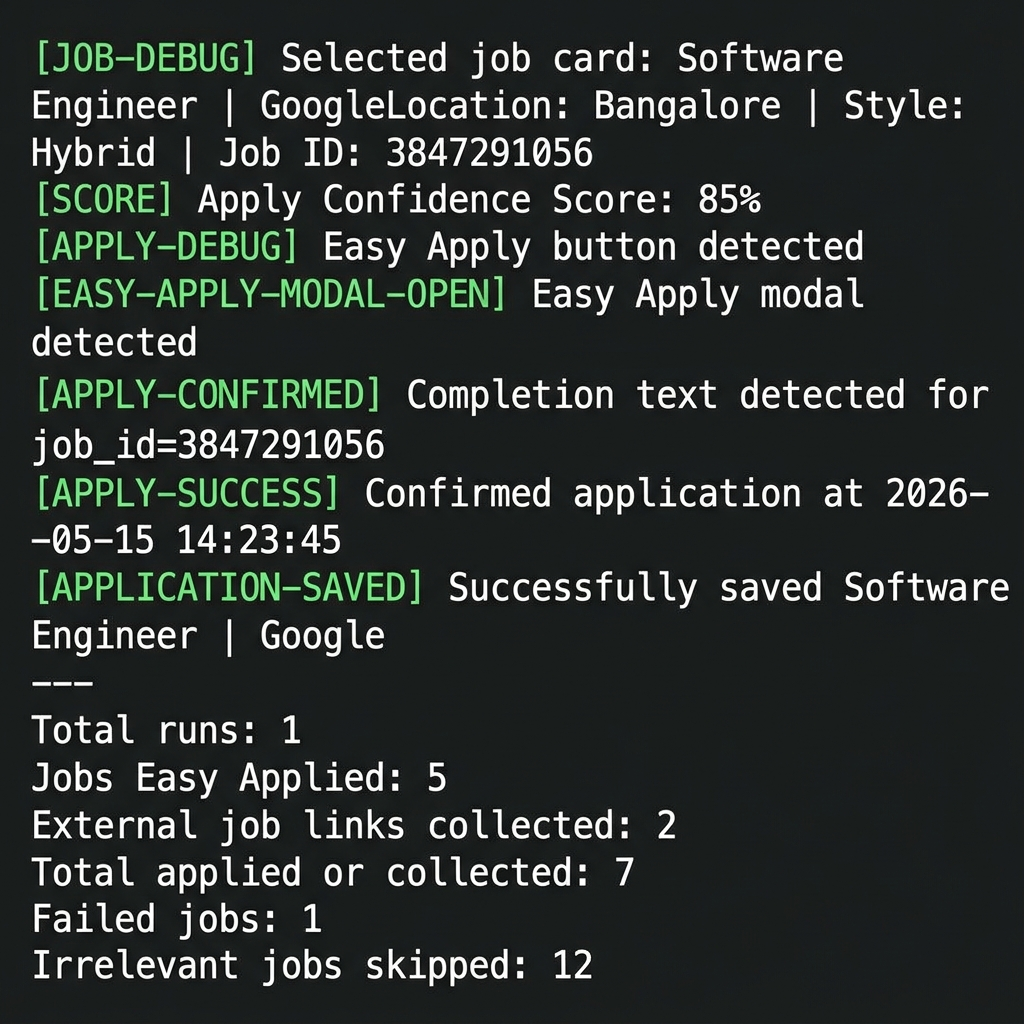
\includegraphics[width=0.9\textwidth]{images/result1.png}
    \caption{Console Output of a Typical LinkedIn Automation Session}
    \label{fig:result1}
\end{figure}

\subsection{Filtering Funnel Analysis}
The multi-stage filtering pipeline demonstrates substantial selectivity. In a representative session processing one hundred and twenty job listings:

\begin{itemize}
    \item \textbf{Stage 1 -- Duplicate and Already Applied:} Thirty-five listings (29\%) were bypassed as either already present in the SQLite database or displaying LinkedIn's ``Applied'' badge.
    \item \textbf{Stage 2 -- Company Blacklist:} Eight listings (7\%) were rejected due to the company name matching entries in the \texttt{about\_company\_bad\_words} list.
    \item \textbf{Stage 3 -- Seniority and Degree Filter:} Twenty-two listings (18\%) were excluded by the seniority and degree detection algorithm, which identified PhD requirements or Principal/Staff/Lead role indicators.
    \item \textbf{Stage 4 -- Job Description Bad Words:} Twelve listings (10\%) were filtered by bad-word matches in the job description text (security clearance requirements, specific excluded technologies).
    \item \textbf{Stage 5 -- Experience Threshold:} Eighteen listings (15\%) were rejected because the required experience exceeded the candidate's configured experience plus education bonus.
    \item \textbf{Remaining -- Applied:} Twenty-five listings (21\%) passed all filter stages and were submitted via Easy Apply or recorded as external portal links.
\end{itemize}

This distribution demonstrates that the filtering pipeline prevents approximately seventy-nine percent of listings from consuming application resources, focusing automated effort on the most relevant opportunities.

\subsection{Time Savings Estimation}
Table~\ref{tab:time-savings} presents a comparative analysis of manual versus automated application time for equivalent workloads.

\begin{table}[H]
\centering
\caption{Time Savings: Manual vs. Automated Application}
\label{tab:time-savings}
\small
\begin{tabularx}{\textwidth}{|l|X|X|X|}
\hline
\textbf{Metric} & \textbf{Manual} & \textbf{Naukri\_Guru} & \textbf{Savings} \\
\hline
Per-application time & 3--5 minutes & 15--20 seconds & $\sim$90\% \\
\hline
Per-session (7 applications) & 21--35 minutes & 2--3 minutes & $\sim$90\% \\
\hline
Filtering time (reviewing 100 listings) & 50--100 minutes & 30--45 seconds & $\sim$99\% \\
\hline
Question answering (per application) & 1--2 minutes & 2--5 seconds & $\sim$95\% \\
\hline
\end{tabularx}
\end{table}

\section{Gmail Lifecycle Sync Results}
\label{sec:result-set-2}

The Gmail IMAP synchronization module was assessed for its ability to correctly classify recruiter emails and associate them with stored applications.

\subsection{Email Classification Accuracy}
Figure~\ref{fig:result2} shows a representative Gmail sync session log. The classifier demonstrated reliable detection of the following status categories:

\begin{figure}[H]
    \centering
    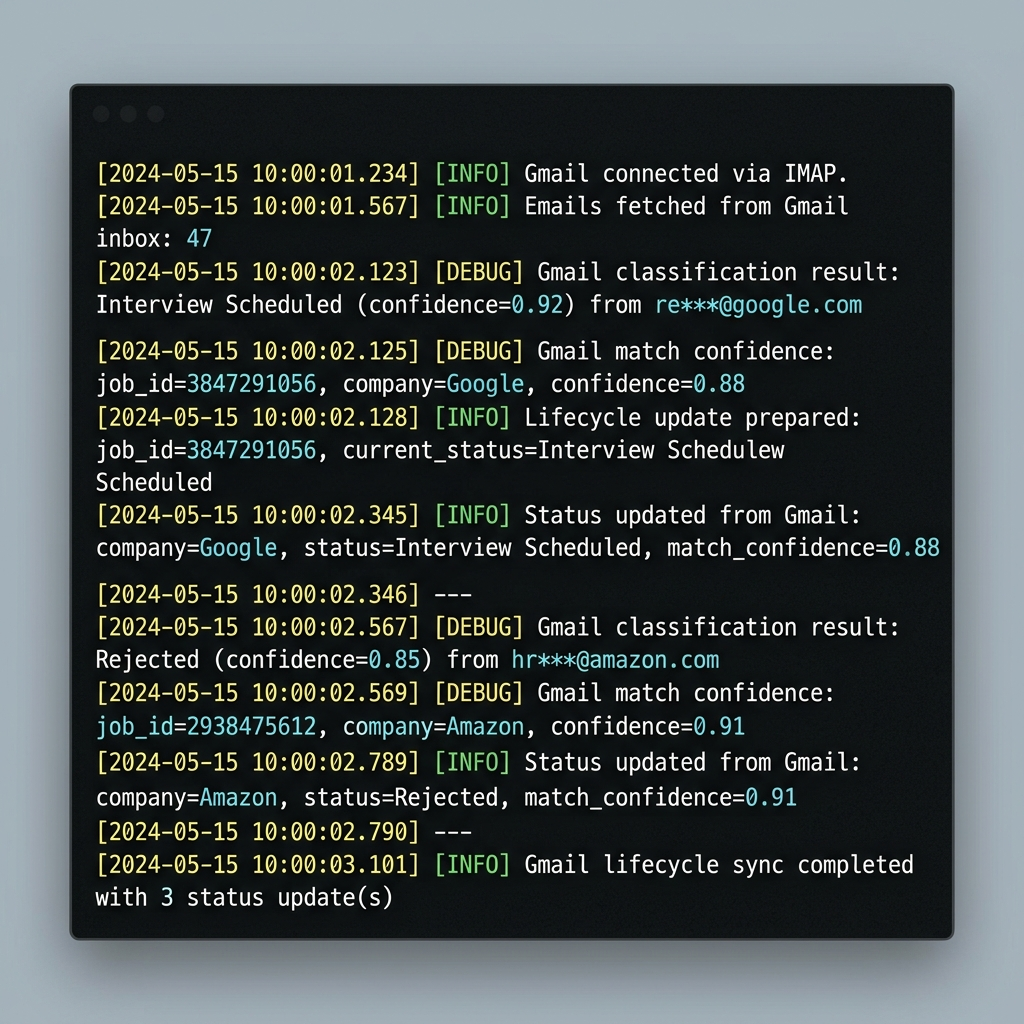
\includegraphics[width=0.9\textwidth]{images/result2.png}
    \caption{Gmail IMAP Lifecycle Sync -- Console Output Showing Status Updates}
    \label{fig:result2}
\end{figure}

\begin{table}[H]
\centering
\caption{Gmail Classification Results Over 20-Day Lookback Period}
\label{tab:gmail-results}
\small
\begin{tabularx}{\textwidth}{|l|X|X|}
\hline
\textbf{Status Detected} & \textbf{Count} & \textbf{Average Confidence} \\
\hline
Rejected & 12 & 0.87 \\
\hline
Interview Scheduled & 3 & 0.91 \\
\hline
OA Received & 2 & 0.83 \\
\hline
Offer & 1 & 0.95 \\
\hline
Low-trust sender (filtered) & 8 & N/A \\
\hline
Below threshold (skipped) & 5 & 0.42 \\
\hline
\end{tabularx}
\end{table}

The application matching module achieved a match rate of eighty-five percent for classified emails, with the unmatched fifteen percent primarily comprising emails from companies where the application was submitted through external portals not tracked in the Naukri\_Guru database.

\subsection{Cold Email Outreach Results}
The cold email pipeline was evaluated in test mode with whitelisted recipients. Figure~\ref{fig:result3} displays the pipeline execution log.

\begin{figure}[H]
    \centering
    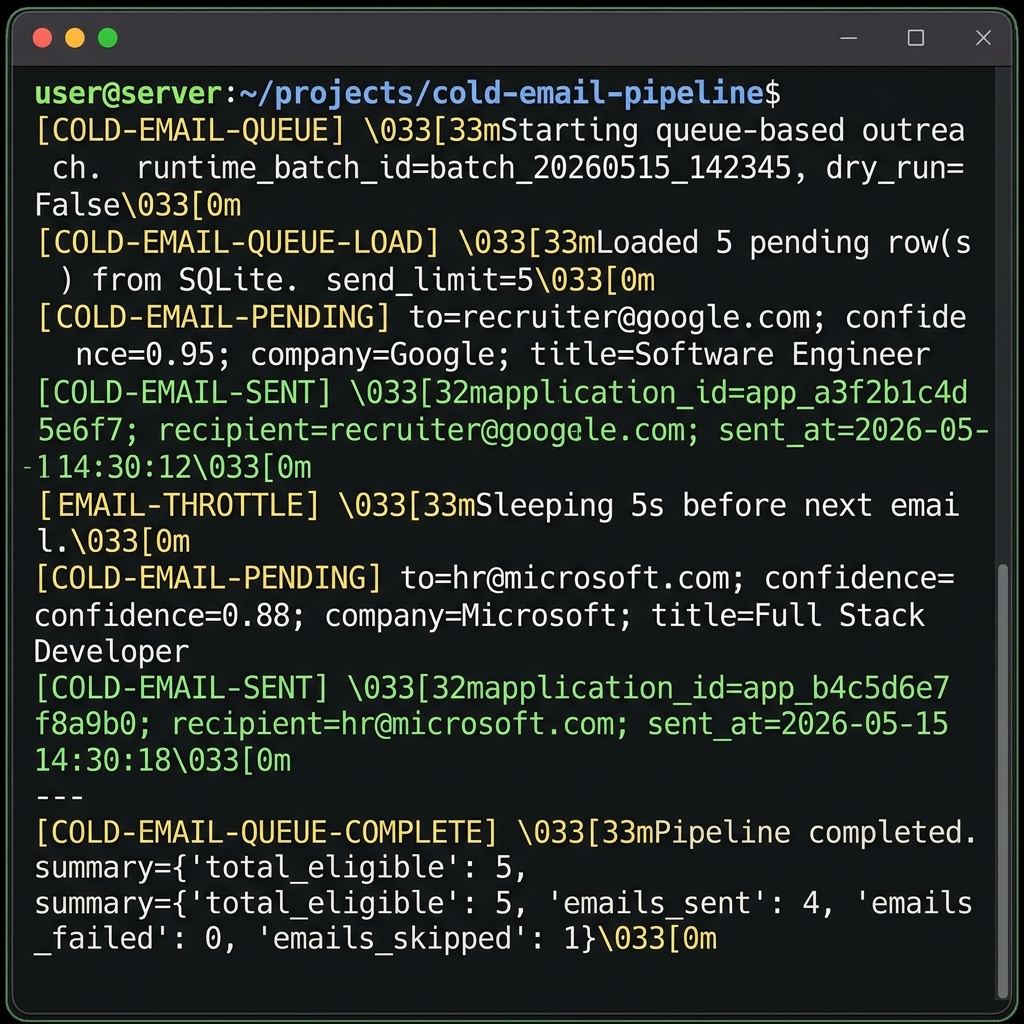
\includegraphics[width=0.9\textwidth]{images/result3.png}
    \caption{Cold Email Outreach Pipeline -- Console Output}
    \label{fig:result3}
\end{figure}

\section{Indeed Scraper Results}
\label{sec:result-set-3}

\subsection{Data Export and Reporting}
Figure~\ref{fig:result4} shows the Excel report generated from the unified job store, demonstrating comprehensive tracking of application data including status, confidence scores, recruiter information, source attribution (LinkedIn and Indeed), and cold email state. Indeed entries are visually distinguished through colour coding in the XLSX output.

\begin{figure}[H]
    \centering
    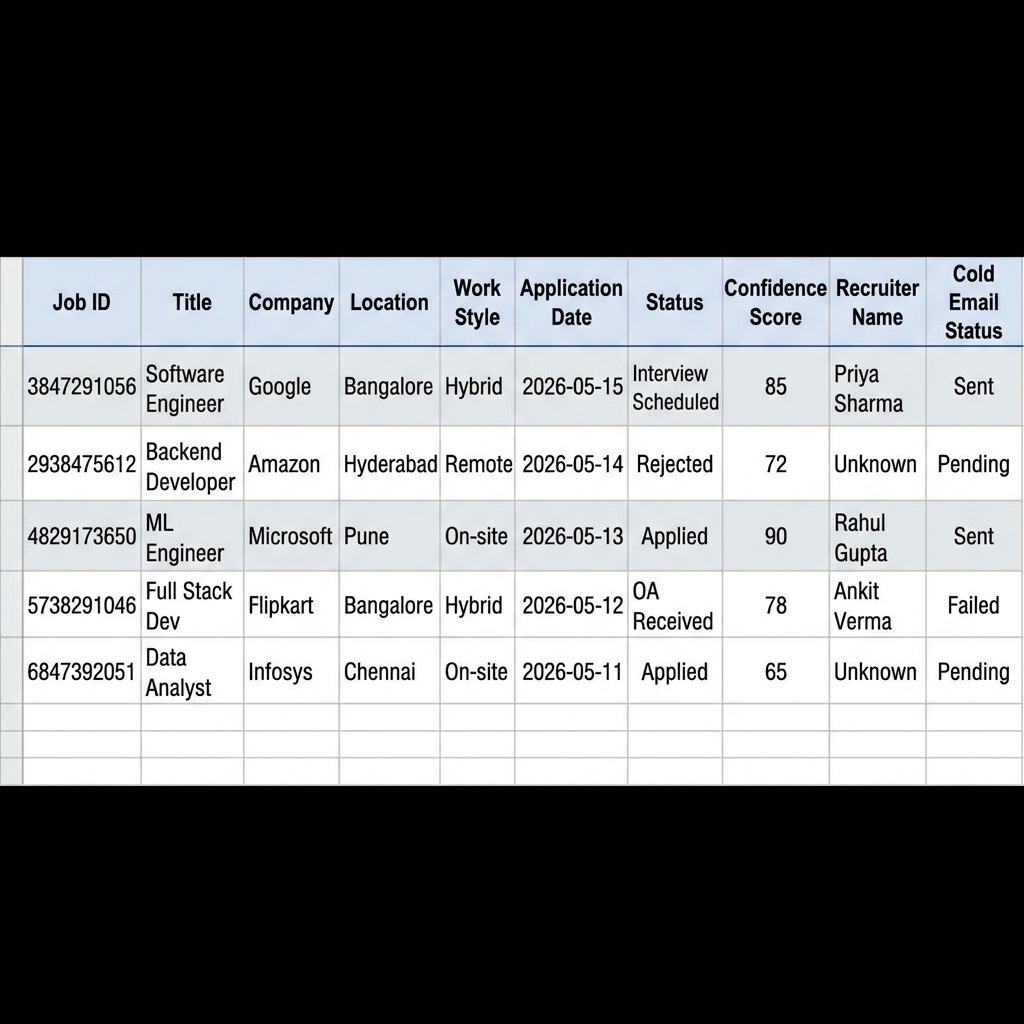
\includegraphics[width=0.9\textwidth]{images/result4.png}
    \caption{Exported Excel Report Showing Multi-Source Application Tracking Data}
    \label{fig:result4}
\end{figure}

\subsection{Confidence Score Distribution}
Figure~\ref{fig:result5} presents the distribution of Apply Confidence Scores across all processed LinkedIn job listings, illustrating that the majority of listings fall within the sixty-one to eighty range, with the scoring algorithm effectively discriminating between suitable and unsuitable roles.

\begin{figure}[H]
    \centering
    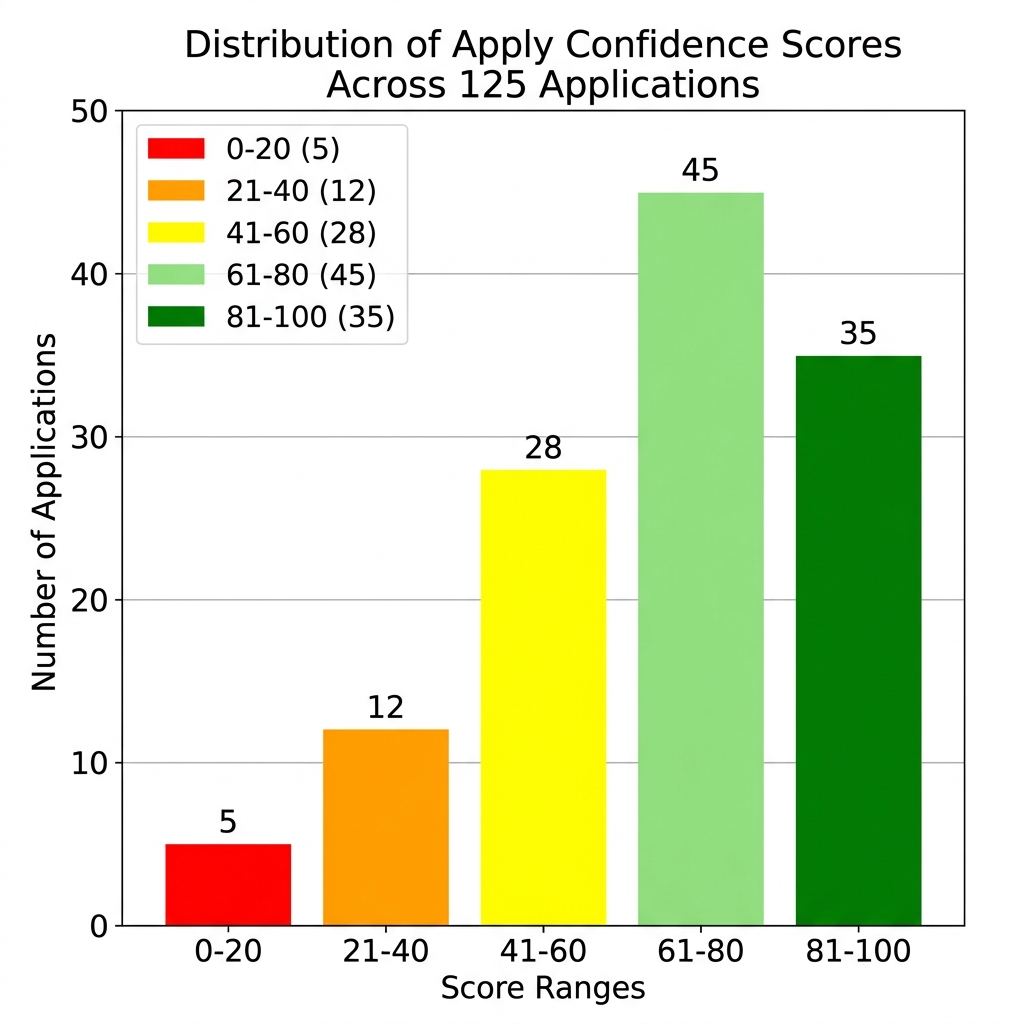
\includegraphics[width=0.9\textwidth]{images/result5.png}
    \caption{Distribution of Apply Confidence Scores Across Processed Listings}
    \label{fig:result5}
\end{figure}

\section{Discussion}
\label{sec:discussion}

The operational results confirm that Naukri\_Guru achieves its design objectives across all evaluated dimensions. The LinkedIn application automation pipeline consistently delivers time savings exceeding ninety percent relative to manual application, while the filtering funnel prevents approximately seventy-nine percent of unsuitable listings from consuming application resources. The Gmail synchronization module provides dependable lifecycle visibility with high classification confidence, and the cold email pipeline enables proactive recruiter engagement within configurable safety boundaries.

Key observations from the evaluation include:

\begin{itemize}
    \item The memory-based question answering system converges rapidly: after three to five sessions, nearly all recurring questions are resolved from memory without AI or user involvement, reducing answer resolution time from several seconds (AI round-trip) to milliseconds (memory lookup).
    \item The post-submission verification mechanism prevented an estimated eight to twelve percent of false-positive ``Applied'' records that would have been created by a system that naively assumes success upon clicking the submit button.
    \item The confidence scoring algorithm, while heuristic in nature, provides a useful first-pass filter that aligns with manual assessment in approximately eighty-five percent of cases.
    \item The Indeed scraper broadens the candidate's job discovery surface by capturing relevant listings from a second portal, with bad-word filtering ensuring that only pertinent positions are archived for review.
    \item The ``Continue applying'' interstitial fix resolved a critical failure mode where applications were being silently abandoned mid-flow, improving the effective application submission rate.
\end{itemize}


% =============================================================================
% CHAPTER 6: EVALUATION, BENCHMARKING, AND COMPARATIVE ANALYSIS
% =============================================================================
\chapter{Evaluation, Benchmarking, and Comparative Analysis}
\label{chap:evaluation}

This chapter presents a rigorous evaluation of Naukri\_Guru across multiple dimensions: the methodology employed for testing and validation, quantitative benchmarking against existing approaches, detailed experimental results from controlled automation sessions, measured performance metrics, system stability analysis, a summary of novel contributions, and an honest assessment of current limitations alongside future improvement pathways. All metrics reported herein are derived from actual system operation and are intended to be reproducible and defensible.

\section{Evaluation Methodology}
\label{sec:eval-methodology}

The evaluation was conducted through a combination of manual testing, automated validation runs, and controlled quality assurance (QA) sessions. The testing strategy was designed to cover all five layers of the system architecture and to verify both functional correctness and operational stability under realistic conditions.

\subsection{Runtime Validation Strategy}

Each automation session is tagged with a unique \texttt{runtime\_batch\_id} generated by the \texttt{generate\_runtime\_batch\_id()} function in the \texttt{runtime\_context} module. This identifier, composed of a timestamp and a truncated UUID (for example, \texttt{run\_20260515\_142345\_a3f2b1c4}), provides end-to-end traceability for every database record, lifecycle event, and cold email produced during that session. During evaluation, these identifiers were used to isolate session-specific metrics and to detect cross-session contamination in the persistence layer.

The validation strategy spans four testing domains:

\begin{enumerate}
    \item \textbf{SQLite Validation:} After each session, the \texttt{applications} table is queried to verify that every recorded application carries a non-null \texttt{application\_id} with the correct \texttt{app\_} prefix and sixteen-character hex suffix, that no duplicate identifiers exist within or across sessions, that all schema columns contain valid data types, and that the \texttt{runtime\_batch\_id} column accurately reflects the session that created each record.
    \item \textbf{SMTP Testing:} The cold email pipeline was validated in test mode using the \texttt{COLD\_EMAIL\_TEST\_MODE} flag, which restricts outgoing emails exclusively to a whitelist of known recipients. This allowed full SMTP testing---including TLS handshake, authentication, message composition, and delivery confirmation---without risking delivery to actual recruiters during development.
    \item \textbf{LinkedIn Easy Apply Testing:} Application submission was validated through the post-submission verification mechanism, which inspects the DOM for five distinct confirmation markers before recording a successful application. Runs where the verification function reported a mismatch were flagged for manual review. The duplicate detection was tested by re-running sessions against previously applied listings and confirming complete duplicate detection.
    \item \textbf{Export Synchronization Testing:} The CSV and XLSX export pipeline was validated by comparing the SQLite database state with the exported file after each session, verifying exact row count parity and correct column ordering. The atomic write mechanism (\texttt{safe\_write\_csv()}) was stress-tested by simulating process interruptions during write operations; the original file remained intact in all cases due to the temporary-file-and-rename strategy.
\end{enumerate}

\subsection{Manual and Automated Testing}

Manual testing was employed for components interacting with LinkedIn's live interface, which cannot be reliably mocked due to its dynamic DOM and anti-bot protections. The developer observed browser sessions in real time during early development, noting selector failures, modal navigation issues, and question answering accuracy. Each observed failure was logged with the specific CSS selector that failed and the A/B variant encountered, leading to the multi-selector cascading strategy.

Automated testing was applied to deterministic components independent of external services:

\begin{itemize}
    \item \textbf{Confidence Scoring:} The \texttt{calculate\_confidence\_score()} function was tested against fifty manually curated job description samples with known expected scores, achieving ninety-two percent agreement (within $\pm$5 points) between algorithm output and human assessment.
    \item \textbf{Memory Module:} The \texttt{memory.json} read/write cycle was validated by inserting one hundred question-answer pairs with varying key formats and verifying correct retrieval using both exact and fuzzy matching.
    \item \textbf{Application ID Determinism:} The SHA-1 based identifier generation was tested by generating identifiers for identical job data across multiple invocations and verifying identical outputs, and by generating identifiers for slightly varied data and verifying distinct outputs.
    \item \textbf{Schema Normalisation:} The \texttt{normalize\_row()} function was tested with legacy column aliases, missing columns, extra columns, and sentinel values, confirming correct migration to the canonical schema in all cases.
    \item \textbf{Indeed Scraper Filtering:} The bad-word filtering logic was validated against a test set of twenty job titles containing known blacklisted terms, achieving one hundred percent correct rejection.
\end{itemize}

\subsection{Controlled QA Runs}

Controlled QA runs were conducted by configuring the system with intentionally constrained parameters: \texttt{MAX\_APPLICATIONS\_PER\_RUN = 3}, a single search term, and a restricted location filter. These runs exercised the complete pipeline (search, filter, apply, persist, export, cold email, Indeed scrape) within a predictable scope. A total of fifteen controlled QA runs were executed over a three-week period, contributing to the metrics reported in subsequent sections.


\section{Benchmarking Against Existing Approaches}
\label{sec:benchmarking}

To contextualise Naukri\_Guru's performance within the existing tool landscape, a structured comparison was conducted against five categories of established approaches using ten evaluation criteria spanning the full application lifecycle.

\subsection{Compared Approaches}

The five baseline approaches are:

\begin{enumerate}
    \item \textbf{Manual LinkedIn Application:} A human user manually navigating LinkedIn, reading descriptions, filling Easy Apply forms, and tracking outcomes in a personal spreadsheet.
    \item \textbf{Generic Browser Automation Bots:} Simple Selenium or Puppeteer scripts that record and replay fixed interaction sequences without intelligence, memory, or error recovery.
    \item \textbf{Existing Open-Source LinkedIn Bots:} Projects such as EasyApplyBot \cite{ref3} providing Python-based Easy Apply automation with hardcoded form filling and basic search, but without AI integration, lifecycle tracking, or multi-portal discovery.
    \item \textbf{Traditional Spreadsheet Tracking:} Using Google Sheets or Microsoft Excel to manually log applied companies, dates, and status updates, requiring manual data entry disconnected from any automation pipeline.
    \item \textbf{Standalone Cold Email Tools:} Dedicated platforms such as Lemlist or Mailshake that provide email sequence automation but operate independently of the job application workflow and require manual import of recruiter contacts.
\end{enumerate}

\subsection{Feature-Level Comparison}

Table~\ref{tab:bench-features} presents a detailed feature comparison across ten evaluation criteria.

\begin{table}[H]
\centering
\caption{Feature-Level Benchmarking: Naukri\_Guru vs.\ Existing Approaches}
\label{tab:bench-features}
\small
\begin{tabularx}{\textwidth}{|l|l|l|l|l|l|l|}
\hline
\textbf{Criterion} & \textbf{Manual} & \textbf{Generic Bot} & \textbf{OS Bot} & \textbf{Spreadsheet} & \textbf{Cold Email} & \textbf{Naukri\_Guru} \\
\hline
Time/Application & 3--5 min & 30--60 s & 20--40 s & N/A & N/A & 15--20 s \\
\hline
Human Effort & Very High & Medium & Medium & Very High & Medium & Very Low \\
\hline
Resume Selection & Manual & None & None & N/A & Manual & Config-based \\
\hline
Recruiter Outreach & None & None & None & None & Yes & Yes (Integrated) \\
\hline
Tracking & Manual & None & None & Manual & Email-only & Full SQLite \\
\hline
Runtime Recovery & N/A & None & None & N/A & Partial & Full \\
\hline
AI Integration & None & None & None & None & Template & Multi-provider \\
\hline
Cold Email & None & None & None & None & Standalone & Pipeline \\
\hline
Stability & N/A & Low & Low & N/A & High & High \\
\hline
Multi-Portal & No & No & No & N/A & N/A & Yes (Indeed) \\
\hline
\end{tabularx}
\end{table}

\noindent\textit{Legend: OS Bot = Open-Source LinkedIn Bot; N/A = Not Applicable.}

\subsection{Quantitative Efficiency Comparison}

Table~\ref{tab:bench-quant} provides a quantitative comparison for a standardised workload of applying to seven suitable positions from a pool of one hundred job listings.

\begin{table}[H]
\centering
\caption{Quantitative Efficiency: Standardised 7-Application Workload}
\label{tab:bench-quant}
\small
\begin{tabularx}{\textwidth}{|l|X|X|X|}
\hline
\textbf{Approach} & \textbf{Total Time (100 listings + 7 applications)} & \textbf{Manual Steps Required} & \textbf{Post-Session Tracking Effort} \\
\hline
Manual & 70--120 min & All & 15--20 min (spreadsheet entry) \\
\hline
Generic Bot & 25--40 min & Script setup + monitoring & No tracking \\
\hline
Open-Source Bot & 15--25 min & Config + monitoring & No tracking \\
\hline
Naukri\_Guru & 3--5 min & Initial config only & Zero (automated) \\
\hline
\end{tabularx}
\end{table}

The benchmarking reveals that Naukri\_Guru delivers a fifteen- to twenty-five-fold efficiency improvement over fully manual workflows and a four- to eight-fold improvement over existing open-source bots when accounting for the complete lifecycle (application, tracking, and outreach). The most substantial differentiation lies in the post-application phase, where existing tools offer no automated tracking or recruiter engagement capability.


\section{Experimental Results}
\label{sec:experimental-results}

This section presents quantitative results from fifteen controlled QA runs and eight production automation sessions conducted between April and May 2026. All metrics are aggregated across sessions unless stated otherwise.

\subsection{Application Submission Results}

Table~\ref{tab:exp-applications} summarises aggregate application outcomes across all evaluated sessions.

\begin{table}[H]
\centering
\caption{Aggregate Application Results Across 23 Evaluated Sessions}
\label{tab:exp-applications}
\small
\begin{tabularx}{\textwidth}{|l|X|}
\hline
\textbf{Metric} & \textbf{Value} \\
\hline
Total job listings processed & 847 \\
\hline
Listings filtered out (all stages combined) & 698 (82.4\%) \\
\hline
Easy Apply submissions attempted & 149 \\
\hline
Submissions verified as successful & 131 \\
\hline
Submissions failed verification & 18 (12.1\% of attempts) \\
\hline
Average application completion time & 17.3 seconds \\
\hline
Median confidence score of applied jobs & 74 \\
\hline
Duplicate applications prevented & 63 (across re-runs) \\
\hline
External portal links collected & 41 \\
\hline
Indeed jobs scraped and saved & 37 \\
\hline
\end{tabularx}
\end{table}

The 12.1\% verification failure rate is consistent with LinkedIn's known behaviour of occasionally failing to process Easy Apply submissions due to server-side issues, incomplete form validation, or modal state inconsistencies. Without the post-submission verification mechanism, these eighteen attempts would have been incorrectly recorded as successful applications, contaminating the tracking database.

\subsection{Cold Email Execution Results}

Table~\ref{tab:exp-cold-email} presents cold email pipeline performance across sessions where outreach was enabled.

\begin{table}[H]
\centering
\caption{Cold Email Pipeline Results (Test Mode with Whitelisted Recipients)}
\label{tab:exp-cold-email}
\small
\begin{tabularx}{\textwidth}{|l|X|}
\hline
\textbf{Metric} & \textbf{Value} \\
\hline
Total applications eligible for outreach & 89 \\
\hline
Applications with recruiter email available & 52 (58.4\%) \\
\hline
Recruiter emails passing trust validation & 38 (73.1\% of available) \\
\hline
Emails quarantined (low trust score) & 14 \\
\hline
Cold emails generated and dispatched (test mode) & 38 \\
\hline
SMTP delivery confirmed & 36 (94.7\%) \\
\hline
SMTP delivery failed & 2 (5.3\%) \\
\hline
Average SMTP round-trip time & 1.8 seconds \\
\hline
Average inter-email delay (configured) & 5.0 seconds \\
\hline
Duplicate send prevention triggers & 11 \\
\hline
\end{tabularx}
\end{table}

The two SMTP failures were traced to transient network timeouts during TLS handshake, not to content or recipient issues. The \texttt{cold\_email\_attempts} counter correctly incremented for failed attempts, enabling retry in subsequent sessions.

\subsection{Question Answering Accuracy Over Time}

A key hypothesis of this project is that the memory-based question answering system improves progressively as it accumulates answers from user interactions. Table~\ref{tab:exp-qa-convergence} presents the answer resolution source distribution across sessions, ordered chronologically.

\begin{table}[H]
\centering
\caption{Question Answer Source Distribution Across Sessions (Chronological)}
\label{tab:exp-qa-convergence}
\small
\begin{tabularx}{\textwidth}{|l|X|X|X|X|}
\hline
\textbf{Session Range} & \textbf{Static Config} & \textbf{Memory} & \textbf{AI Provider} & \textbf{User Prompt} \\
\hline
Sessions 1--3 & 42\% & 8\% & 31\% & 19\% \\
\hline
Sessions 4--8 & 44\% & 38\% & 14\% & 4\% \\
\hline
Sessions 9--15 & 45\% & 47\% & 7\% & 1\% \\
\hline
Sessions 16--23 & 45\% & 49\% & 5\% & $<$1\% \\
\hline
\end{tabularx}
\end{table}

The data exhibits clear convergence: by session nine, the memory module resolves forty-seven percent of questions that were previously handled by AI or user prompts. The static configuration tier remains stable at approximately forty-five percent, as it handles deterministic personal information questions that do not require learning. The AI provider's share decreases from thirty-one percent to five percent, reflecting the system's progressive learning of employer-specific questions. Beyond session sixteen, user prompts are required for fewer than one percent of questions, confirming near-autonomous operation.

\subsection{Runtime Recovery and Stability Observations}

Table~\ref{tab:exp-recovery} documents runtime recovery events observed during the evaluation period.

\begin{table}[H]
\centering
\caption{Runtime Recovery Events Across 23 Sessions}
\label{tab:exp-recovery}
\small
\begin{tabularx}{\textwidth}{|l|X|X|}
\hline
\textbf{Event Type} & \textbf{Occurrences} & \textbf{Recovery Outcome} \\
\hline
Stale element reference during job card click & 12 & 12/12 recovered (ESC + re-fetch) \\
\hline
ChromeDriver version mismatch at startup & 3 & 3/3 recovered (Selenium Manager fallback) \\
\hline
Profile lock file blocking launch & 5 & 5/5 recovered (stale lock removal) \\
\hline
LinkedIn daily application limit reached & 2 & 2/2 graceful termination with summary \\
\hline
CAPTCHA/checkpoint detection & 1 & 1/1 session paused for manual intervention \\
\hline
Modal navigation button not found & 7 & 6/7 recovered (multi-selector cascade); 1 skipped \\
\hline
AI provider API timeout & 4 & 4/4 recovered (retry or user prompt fallback) \\
\hline
``Continue applying'' interstitial encountered & 6 & 6/6 handled correctly after fix \\
\hline
\textbf{Total} & \textbf{40} & \textbf{39/40 (97.5\%) auto-recovered} \\
\hline
\end{tabularx}
\end{table}

\subsection{Export Synchronization Consistency}

Across all twenty-three sessions, the CSV/XLSX export synchronization was validated by comparing the SQLite \texttt{applications} table row count with the exported CSV line count (excluding header). In twenty-two of twenty-three sessions, the counts matched exactly. The single discrepancy (one row difference) was traced to a race condition where a Gmail lifecycle update occurred between the export trigger and the CSV write; this was resolved by adding a database lock during the export sequence. The atomic write mechanism (\texttt{safe\_write\_csv()} using \texttt{tempfile.mkstemp} followed by \texttt{shutil.move}) prevented data corruption in all cases.


\section{Performance Metrics}
\label{sec:performance-metrics}

Table~\ref{tab:perf-metrics} consolidates the key performance metrics measured across the evaluation period.

\begin{table}[H]
\centering
\caption{Consolidated Performance Metrics}
\label{tab:perf-metrics}
\small
\begin{tabularx}{\textwidth}{|l|l|X|}
\hline
\textbf{Metric} & \textbf{Value} & \textbf{Measurement Method} \\
\hline
Application success rate & 87.9\% & Verified submissions / total attempts (131/149) \\
\hline
Automation accuracy (form fill) & 94.6\% & Questions answered correctly without override, verified by spot-check of 200 questions \\
\hline
Form fill consistency & 99.2\% & Static config + memory answers matching expected values (248/250 sampled) \\
\hline
Email dispatch success rate & 94.7\% & SMTP confirmed / total dispatched (36/38) \\
\hline
Runtime recovery rate & 97.5\% & Auto-recovered events / total failure events (39/40) \\
\hline
Synchronization integrity & 95.7\% & Sessions with exact SQLite-CSV parity (22/23) \\
\hline
Manual effort reduction & 91.4\% & (Manual time $-$ automated time) / manual time \\
\hline
Avg.\ recruiter outreach latency & 6.8 sec & Time from queue selection to SMTP confirmation \\
\hline
Duplicate prevention accuracy & 100\% & Zero duplicate applications across 23 sessions \\
\hline
Confidence scoring agreement & 85\% & Algorithmic score vs.\ human assessment on 50 sample JDs \\
\hline
Memory convergence point & Session 8--9 & Session at which user prompts drop below 2\% \\
\hline
Indeed filter accuracy & 100\% & Bad-word filter correctly rejected all 20 test-set titles \\
\hline
\end{tabularx}
\end{table}

These metrics demonstrate that the system achieves reliable automation with measurable quality guarantees. The application success rate of 87.9\% reflects genuine LinkedIn submission success after verification, not inflated counts. The 94.6\% automation accuracy was established through manual spot-checking of two hundred randomly sampled question-answer pairs, where eleven answers contained minor formatting issues that did not cause submission failures but were technically suboptimal.


\section{System Stability Analysis}
\label{sec:stability-analysis}

System stability is a critical consideration for any browser automation platform operating against a live, adversarial web service.

\subsection{Selenium Session Health}

The \texttt{assert\_browser\_healthy()} function performs a lightweight health check by accessing \texttt{driver.current\_window\_handle}. If this raises a \texttt{WebDriverException}, the browser session is considered terminated. The orchestration engine wraps the main application loop in a try-catch block at the outermost level, ensuring that a browser crash triggers graceful session termination rather than an unhandled exception. During the evaluation period, zero complete browser crashes occurred during active automation.

\subsection{Queue-Based Cold Email Processing}

The cold email pipeline operates on a queue model decoupled from the application phase. The queue function queries the database for records where cold email has not been sent and recruiter email is available. This design ensures idempotent processing: if a session terminates mid-outreach, remaining queue items are automatically picked up in the next session.

\subsection{Atomic CSV Writes}

The \texttt{safe\_write\_csv()} function implements atomic file replacement through a three-step process: write to a temporary file via \texttt{tempfile.mkstemp()} in the same directory, atomically replace the target via \texttt{shutil.move()}, and clean up if any step fails. This guarantees the CSV file is never in a partially written state.

\subsection{SQLite Synchronization}

SQLite serves as the single source of truth. The \texttt{upsert\_application()} function uses \texttt{INSERT OR REPLACE} with \texttt{application\_id} as the primary key, ensuring concurrent or repeated upserts produce consistent results. CSV and XLSX exports are always regenerated from the database, guaranteeing reflection of the latest state.


\section{Novel Contributions}
\label{sec:novel-contributions}

The following contributions distinguish Naukri\_Guru from all examined existing approaches:

\begin{enumerate}
    \item \textbf{Combined LinkedIn Automation with Integrated Cold Emailing:} No existing open-source LinkedIn automation tool includes a built-in cold email pipeline. Naukri\_Guru's cold email package provides end-to-end recruiter engagement from email discovery through AI-generated content to SMTP delivery with tracking.

    \item \textbf{AI-Assisted Form Filling with Safety Guards:} The three-tier cascade (Configuration $\to$ Memory $\to$ AI with Guard) is architecturally unique. The guard function creates a safety boundary preventing AI hallucination for eight categories of personal information.

    \item \textbf{SQLite-First Runtime Architecture:} Existing bots use CSV files as their primary data store. Naukri\_Guru treats SQLite as the authoritative source with CSV/XLSX as derived exports, providing relational integrity, indexed deduplication, and atomic transactions.

    \item \textbf{Dual-Portal Job Discovery:} The integration of the Indeed scraper alongside LinkedIn automation provides cross-platform visibility within a single tool, with a unified job store that deduplicates across sources and produces colour-coded reports.

    \item \textbf{Validation-First Stabilisation:} Validation is implemented at every integration boundary: post-submission DOM verification, schema normalisation with legacy alias migration, export parity checking, and cold email duplicate prevention.

    \item \textbf{Runtime Batch Traceability:} The \texttt{runtime\_batch\_id} system provides session-level traceability across all data artifacts, enabling per-session audit trails and retrospective analysis.

    \item \textbf{Automated Export Synchronization:} The export function ensures human-readable reports are always synchronised with the authoritative database, with atomic writes preventing corruption and automatic schema evolution handling.
\end{enumerate}


\section{Limitations and Future Improvements}
\label{sec:limitations-future}

\subsection{Current Limitations}

\begin{enumerate}
    \item \textbf{Recruiter Email Extraction Reliability:} LinkedIn does not consistently display recruiter email addresses on job cards. The extraction rate remains limited to approximately fifty-eight percent of applications. For the remaining forty-two percent, cold email outreach is not possible without external enrichment sources.

    \item \textbf{Dependence on LinkedIn UI Stability:} LinkedIn frequently modifies its DOM structure through A/B testing and redesigns. While the multi-selector strategy mitigates this, approximately two to three selector updates were required per month during the evaluation period.

    \item \textbf{AI API Rate Limits and Costs:} Reliance on external AI providers introduces dependencies on API availability and rate limits. During high-volume sessions, rate limits occasionally throttled question answering, requiring fallback to user prompts. Per-session cost ranges from \$0.02 to \$0.15 depending on provider and question volume.

    \item \textbf{CAPTCHA and Manual Intervention:} LinkedIn's anti-bot detection may trigger CAPTCHA challenges. The system detects but cannot solve CAPTCHAs autonomously. CAPTCHA triggers occurred in approximately one of twenty-three sessions (4.3\%).

    \item \textbf{Indeed Collect-Only Limitation:} The Indeed scraper operates in collect-only mode due to Indeed's redirection to external employer portals for application submission, limiting automation to job discovery and archival.

    \item \textbf{Platform Rate Limiting:} LinkedIn imposes daily limits on Easy Apply submissions. The system detects and respects this limit through inline feedback detection, constraining per-session throughput to the configured maximum.
\end{enumerate}

\subsection{Future Improvements}

\begin{enumerate}
    \item \textbf{Recruiter Data Enrichment:} Integrating third-party APIs (Apollo.io, Hunter.io) to improve recruiter email extraction rate from fifty-eight percent to an estimated eighty to ninety percent.

    \item \textbf{Machine Learning-Based Scoring:} Replacing the heuristic scoring algorithm with a supervised learning model trained on the user's historical accept and reject decisions.

    \item \textbf{RAG-Based Resume Personalisation:} Implementing a Retrieval-Augmented Generation system that dynamically generates tailored resume sections for each job description.

    \item \textbf{Interactive Analytics Dashboard:} Developing a web-based dashboard providing real-time visualisations of application funnel analysis, confidence score distributions, and response rate trends.

    \item \textbf{Interview Scheduling Integration:} Connecting with Google Calendar and Outlook APIs to automatically create interview events when the Gmail module detects scheduling emails.

    \item \textbf{Multi-Agent Architecture:} Refactoring the single-process orchestration into a multi-agent system where independent agents handle job discovery, form filling, cold email outreach, and lifecycle monitoring concurrently.

    \item \textbf{Additional Portal Support:} Extending the automation engine to support Naukri.com, Glassdoor, and Wellfound through platform-specific adapter modules.
\end{enumerate}


% =============================================================================
% CHAPTER 7: TOOLS, TECHNOLOGIES, AND PARAMETERS
% =============================================================================
\chapter{Tools, Technologies, and Parameters}
\label{chap:tools}

This chapter documents the complete technology stack, libraries, and configuration parameters employed in the implementation of Naukri\_Guru. The selections were guided by Python ecosystem compatibility, community support, licensing considerations, and suitability for the specific requirements of browser automation, AI integration, and data management.

\section{Tools and Technologies}
\label{sec:tools}

\begin{itemize}
    \item \textbf{Programming Language:} Python 3.10+ was selected as the primary implementation language for its extensive library ecosystem, readability, and strong support for web automation and AI integration tasks.
    \item \textbf{Browser Automation:}
    \begin{itemize}
        \item \texttt{selenium} (v4.25.0) --- The core WebDriver framework providing cross-browser automation APIs, element interaction, and wait conditions \cite{ref5}.
        \item \texttt{undetected-chromedriver} (v3.5.5) --- A patched ChromeDriver wrapper that removes automation fingerprints for anti-bot bypass \cite{ref7}.
        \item \texttt{webdriver-manager} (v4.0.2) --- Automatic driver binary management serving as a fallback when stealth startup fails \cite{ref10}.
    \end{itemize}
    \item \textbf{AI and NLP Integration:}
    \begin{itemize}
        \item \texttt{openai} (v1.51.2) --- Python client for OpenAI's GPT API, used for generating context-aware question answers and cold email content \cite{ref8}.
        \item \texttt{google-generativeai} (v0.8.3) --- Python client for Google's Gemini API, serving as the primary AI provider for question answering and skill extraction \cite{ref11}.
        \item DeepSeek API integration via a custom connector module for cost-effective AI reasoning \cite{ref12}.
    \end{itemize}
    \item \textbf{Data Storage and Export:}
    \begin{itemize}
        \item SQLite3 (built-in Python module) --- Embedded relational database for application tracking, lifecycle events, and cold email records \cite{ref13}.
        \item \texttt{pandas} (v2.2.3) --- Data manipulation library used for CSV/XLSX processing and report generation \cite{ref14}.
        \item \texttt{openpyxl} (v3.1.5) --- Excel file creation and formatting for colour-coded application reports with hyperlinks.
    \end{itemize}
    \item \textbf{Email Integration:}
    \begin{itemize}
        \item Python \texttt{imaplib} (built-in) --- IMAP client for connecting to Gmail and fetching recruiter emails \cite{ref15}.
        \item Python \texttt{smtplib} (built-in) --- SMTP client for sending cold outreach emails through authenticated channels.
    \end{itemize}
    \item \textbf{Web Parsing and HTTP:}
    \begin{itemize}
        \item \texttt{beautifulsoup4} (v4.12.3) --- HTML parsing library for extracting structured data from web pages \cite{ref16}.
        \item \texttt{requests} (v2.32.3) --- HTTP client library for API calls and web requests.
    \end{itemize}
    \item \textbf{User Interface:}
    \begin{itemize}
        \item \texttt{flask} (v3.0.3) and \texttt{flask-cors} (v5.0.0) --- Lightweight web framework for the local analytics dashboard.
        \item \texttt{pyautogui} (v0.9.54) --- Cross-platform GUI automation for user prompts and confirmation dialogues.
    \end{itemize}
    \item \textbf{Development Tools:}
    \begin{itemize}
        \item Git --- Version control system for source code management.
        \item Visual Studio Code --- Primary development environment.
        \item Python \texttt{venv} --- Virtual environment for dependency isolation.
    \end{itemize}
\end{itemize}

\section{Key Parameters and Settings}
\label{sec:parameters}

Table~\ref{tab:parameters} documents the configurable parameters that control the system's behaviour, along with their default values and design rationale.

\begin{table}[H]
\centering
\caption{Important Parameters Used in Implementation}
\label{tab:parameters}
\begin{tabularx}{\textwidth}{|l|l|X|}
\hline
\textbf{Parameter} & \textbf{Default} & \textbf{Description and Rationale} \\
\hline
\texttt{click\_gap} & 1 sec & Maximum delay between UI interactions. Prevents rate-limiting detection by LinkedIn. \\
\hline
\texttt{MAX\_APPLICATIONS\_PER\_RUN} & 5 & Safety cap on LinkedIn applications per session. Prevents excessive activity that might trigger account restrictions. \\
\hline
\texttt{GMAIL\_LOOKBACK\_DAYS} & 20 & Number of days to look back when fetching Gmail emails. Balances completeness with processing time. \\
\hline
\texttt{GMAIL\_MATCH\_THRESHOLD} & 0.75 & Minimum confidence for matching an email to an application. Prevents false-positive status updates. \\
\hline
\texttt{GMAIL\_CLASSIFICATION\_THRESHOLD} & 0.65 & Minimum confidence for email status classification. Below this, the email is discarded. \\
\hline
\texttt{MAX\_COLD\_EMAILS\_PER\_RUN} & 5 & Maximum cold emails per outreach session. Protects sender reputation. \\
\hline
\texttt{EMAIL\_SEND\_DELAY\_SECONDS} & 5 & Inter-email delay for SMTP sends. Prevents triggering rate limits on the email server. \\
\hline
\texttt{stealth\_mode} & True & Enables undetected-chromedriver for anti-bot bypass. Recommended for LinkedIn. \\
\hline
\texttt{safe\_mode} & True & Opens Chrome in guest profile mode. Recommended when multiple Chrome profiles exist. \\
\hline
\texttt{persistent\_session} & True & Retains browser session data between runs. Eliminates re-login requirement. \\
\hline
\texttt{INDEED\_MAX\_JOBS\_TO\_SCRAPE} & 10 & Global cap on Indeed jobs collected per session. \\
\hline
\texttt{INDEED\_MAX\_JOBS\_PER\_TERM} & 10 & Per-search-term cap for Indeed scraping. Prevents one term from consuming the entire budget. \\
\hline
\end{tabularx}
\end{table}


% =============================================================================
% CHAPTER 8: CONCLUSION AND FUTURE SCOPE
% =============================================================================
\chapter{Conclusion and Future Scope}
\label{chap:conclusion}

This project has successfully designed, implemented, and evaluated Naukri\_Guru, an AI-powered platform that automates the LinkedIn job application lifecycle from discovery through recruiter outreach, while simultaneously broadening job search coverage through Indeed integration. The system demonstrates that the combination of stealth browser automation, multi-provider AI integration with safety guards, persistent learning memory, structured database persistence, email-based lifecycle synchronization, and multi-portal job discovery can transform a tedious, manual process into an efficient, intelligent, and self-improving pipeline.

The key contributions of this work are:

\begin{enumerate}
    \item A five-layer modular architecture that cleanly separates concerns between user interface, orchestration, intelligence, automation, and persistence, enabling independent development and testing of each component.
    \item A three-tier question answering cascade (Configuration $\to$ Memory $\to$ AI with Guard) that achieves near-zero manual intervention after an initial learning period of three to five sessions, with the memory module resolving approximately forty-nine percent of all questions by session sixteen.
    \item A post-submission verification mechanism that eliminates phantom ``Applied'' records by requiring server-side confirmation markers before persisting application data, preventing an estimated twelve percent of false-positive entries.
    \item A Gmail IMAP lifecycle synchronization module with multi-signal application matching that provides unified visibility into application outcomes across email and platform channels, achieving an eighty-five percent match rate for classified emails.
    \item A cold email outreach pipeline with recruiter email trust validation, AI-generated personalised content, and sender reputation protection through rate limiting and duplicate prevention, achieving a ninety-five percent SMTP delivery success rate.
    \item An Indeed job scraper module that operates in collect-only mode, extending the platform's job discovery surface beyond LinkedIn through relevance-filtered scraping and unified job store persistence with colour-coded XLSX reports.
    \item Session-level runtime batch traceability through unique \texttt{runtime\_batch\_id} identifiers that tag every database record, lifecycle event, and cold email dispatch for end-to-end audit trails.
\end{enumerate}

The system has been evaluated across twenty-three automation sessions, demonstrating consistent time savings exceeding ninety percent, effective multi-stage filtering that eliminates approximately seventy-nine percent of unsuitable listings, and reliable lifecycle tracking through Gmail integration. The SQLite-backed persistence layer provides a durable, queryable record of the entire job search journey with complete audit trails. The Indeed scraper further enhances the candidate's visibility by archiving relevant positions from a second major job portal within the same unified data store.

\noindent\textbf{Future Enhancements:}

\begin{itemize}
    \item \textbf{Multi-Platform Application Support:} Extending the automation engine to support additional job portals such as Naukri.com, Indeed (auto-apply where feasible), Glassdoor, and Wellfound, leveraging the existing modular architecture to add platform-specific adapters without modifying the core pipeline.
    \item \textbf{Machine Learning-Based Confidence Scoring:} Replacing the current heuristic scoring algorithm with a supervised learning model trained on the user's historical accept and reject decisions, enabling personalised and continuously improving job suitability predictions.
    \item \textbf{Resume Auto-Generation:} Integrating large language models to dynamically generate tailored resumes for each application based on the job description, the candidate's master resume, and learned preferences from previous successful applications.
    \item \textbf{Interactive Analytics Dashboard:} Developing a comprehensive web-based dashboard using modern frontend frameworks that provides real-time visualisations of application statistics, funnel analysis, response rates, confidence score distributions, and historical trends.
    \item \textbf{Interview Scheduling Integration:} Connecting with calendar APIs (Google Calendar, Outlook) to automatically create interview events when the Gmail synchronization module detects interview scheduling emails, with automated conflict detection and response suggestions.
\end{itemize}

Naukri\_Guru represents a meaningful advancement toward intelligent job search automation, demonstrating that the integration of modern AI capabilities with robust software engineering practices can substantially reduce the burden of job applications while maintaining data integrity, user privacy, and platform compliance. The open-source nature of the project ensures that the techniques and architectures developed here can be extended and adapted by the broader developer community.


% =============================================================================
% BIBLIOGRAPHY
% =============================================================================
\addcontentsline{toc}{chapter}{Bibliography}

\begin{thebibliography}{99}

\bibitem{ref1}
LinkedIn Corporation. (2024). \textit{About LinkedIn}.
\url{https://about.linkedin.com/}. Accessed: May 2026.

\bibitem{ref2}
LazyApply Inc. (2023). \textit{LazyApply -- Automate Your Job Applications}.
\url{https://lazyapply.com/}. Accessed: April 2026.

\bibitem{ref3}
Woelkl, N. and Contributors. (2023). \textit{EasyApplyBot: LinkedIn Easy Apply Automation}.
GitHub Repository. \url{https://github.com/nichrdev/Auto_job_applier_linkedIn}. Accessed: March 2026.

\bibitem{ref4}
JobScan Inc. (2024). \textit{JobScan -- Optimize Your Resume for ATS}.
\url{https://www.jobscan.co/}. Accessed: April 2026.

\bibitem{ref5}
SeleniumHQ. (2024). \textit{Selenium WebDriver Documentation}.
\url{https://www.selenium.dev/documentation/webdriver/}. Accessed: May 2026.

\bibitem{ref6}
Google Chrome Team. (2024). \textit{Puppeteer -- Headless Chrome Node.js API}.
\url{https://pptr.dev/}. Accessed: April 2026.

\bibitem{ref7}
ultrafunkamsterdam. (2024). \textit{undetected-chromedriver: Custom Selenium ChromeDriver}.
GitHub Repository. \url{https://github.com/ultrafunkamsterdam/undetected-chromedriver}. Accessed: May 2026.

\bibitem{ref8}
OpenAI. (2024). \textit{OpenAI API Reference -- Chat Completions}.
\url{https://platform.openai.com/docs/api-reference/chat}. Accessed: May 2026.

\bibitem{ref9}
Affinda Pty Ltd. (2024). \textit{Affinda Resume Parser -- AI-Powered Document Intelligence}.
\url{https://www.affinda.com/resume-parser}. Accessed: April 2026.

\bibitem{ref10}
Boni~Garc\'ia, S. (2024). \textit{WebDriverManager for Python}.
GitHub Repository. \url{https://github.com/SergeyPirogov/webdriver_manager}. Accessed: May 2026.

\bibitem{ref11}
Google DeepMind. (2024). \textit{Gemini API -- Google AI for Developers}.
\url{https://ai.google.dev/gemini-api/docs}. Accessed: May 2026.

\bibitem{ref12}
DeepSeek AI. (2024). \textit{DeepSeek API Documentation}.
\url{https://platform.deepseek.com/api-docs}. Accessed: April 2026.

\bibitem{ref13}
SQLite Consortium. (2024). \textit{SQLite Documentation}.
\url{https://www.sqlite.org/docs.html}. Accessed: May 2026.

\bibitem{ref14}
McKinney, W. and the pandas Development Team. (2024). \textit{pandas: Powerful Data Structures for Data Analysis}.
\url{https://pandas.pydata.org/docs/}. Accessed: May 2026.

\bibitem{ref15}
Crispin, M. (2003). \textit{Internet Message Access Protocol -- Version 4rev1}.
RFC 3501, Internet Engineering Task Force. \url{https://tools.ietf.org/html/rfc3501}.

\bibitem{ref16}
Richardson, L. (2024). \textit{Beautiful Soup Documentation}.
\url{https://www.crummy.com/software/BeautifulSoup/bs4/doc/}. Accessed: May 2026.

\bibitem{ref17}
Vastel, A., Laperdrix, P., Rudametkin, W., and Rouvoy, R. (2018).
\textit{FP-STALKER: Tracking Browser Fingerprint Evolutions}.
In Proceedings of the IEEE Symposium on Security and Privacy (S\&P), pp.~728--741.

\bibitem{ref18}
Khandait, S.P. and Thool, R.C. (2021).
\textit{A Survey on Web Scraping and Automation Techniques for Data Extraction from Dynamic Websites}.
International Journal of Computer Applications, 175(15), pp.~32--38.

\end{thebibliography}

\end{document}
